
\include{JIBLM}

%
%%%%%%%%%%%%%%%%%%%%% Annotation Environment Switch%%%%%%%%%%%%
%\StudentVersion
\InstructorVersion
%%%%%%%%%%%%%%%%%%%%% Annotation Environment Switch%%%%%%%%%%%%
%

\newcommand\bq{\begin{question}}
\newcommand\eq{\end{question}}
\newcommand\be{\begin{enumerate}}
\newcommand\ee{\end{enumerate}}
\renewcommand{\labelenumi}{\alph{enumi})}


\begin{document}
\large
\frontmatter
\title{Math 139: \\ Plane Analytic Geometry \\ Notes and Problems}
\author{Nicholas Long}
\affiliation{SFASU}
\maketitle
%\tableofcontents

\begin{annotation}
\chapter{To the Instructor}
I wrote much of this introduction, as well as the instructor comments within the notes, in order to highlight some of the ideas that have worked well for me and the other professor who has used these notes. As always with materials for the classroom, your results will vary. A guiding principle of active classrooms is to do what you think works best. Many of the ideas stated here may be familiar to instructors experienced in running an inquiry oriented classroom, but I feel compelled to restate them for clarity.
This introduction describes the implementation of these notes within the pre-calculus level Plane Analytic Geometry course for which they were written, including successes, difficulties, and characteristics of the student population. I have also included some grading rubrics and other variations that I have used. On certain problems, I have added superscripts leading to comments in the endnotes in the last chapter, “Notes to the Instructor.”

\section{Course Background}
These notes were developed for use in a pre-calculus level Plane Analytic Geometry course at Stephen F. Austin State University (SFA). SFA is a medium-sized, comprehensive, regional state university in East Texas, with a mathematics and statistics department that graduates about 20 to 30 mathematics majors each year. This geometry course is the third in a sequence of courses used for calculus preparation. The prerequisite courses are College Algebra and Trigonometry, both of which have a fairly standard set of content but are not typically taught outside of a lecture model with some active learning ideas (like think-pair-share) used at the instructors discretion. Whereas the College Algebra and Trigonometry courses are typically taught by Instructors, the Plane Analytic Geometry course is almost always taught by tenure track faculty. This course is often seen by faculty at SFA as an opportunity for students to gain mathematical maturity before calculus. These notes have been used in five different sections (including a five week summer semester) over four years by two faculty members. The sections in which these notes were used varied from 13 to 30 students, with the greatest success around 20 students.

These notes were designed to grow the mathematical maturity of students, to help students understand mathematical notation, and to have students connect the geometric elements they have studied with the algebraic skills they have practiced. Part of this growth comes from deeper examination of a few examples (or sometimes just one), rather than exposing students to as many exercises as possible. In particular, students can often be successful in previous courses through mimicry of examples from resources like lecture notes, textbooks, and the internet, but they are missing how a skill they practiced is useful outside of the section of material. By stripping away as many of the traditional resources as possible and pairing down the voluminous amount of exercises a student is expected to do, these notes aim to have students connect ideas from this and previous courses to solve problems. Clear and efficient communication as well as persistence are meta-goals of this approach to the course. In particular, persistence in problem solving is grown throughout this problem set, through the use of scaffolding early on and more open ended problems or questions without explicit intermediate steps in the later stages of the course.

These notes are constructed as a mix of calculation, examples/counter-examples, and conjecture that are meant to guide students through basic precalculus geometric objects, transformations, and measurements on a two-dimensional plane with an emphasis on connections to previous ideas. For example, students likely have seen much of the material in the first chapter of the notes (coordinates, lines, vectors, etc.) from their previous course work. These notes however emphasize developing an understanding of connections between ideas as well as the cultivation of productive habits of mind. From a pedagogical standpoint, this means focusing on individual student growth. Specifically, many students have a poor understanding of when and how they achieve mastery of material. As such, these notes center on helping students see the difference between being able to work through a few examples and being able to move easily between general and specific cases. A typical development of a topic involves presenting some definition, working through a scaffolded set of steps to understand the first examples, then generalizing the topic and finally applying that generalization to another example. Sometimes a future area of work is previewed. The examples are presented in such a way that the details are almost always developed by students and typically selected in order to represent \textit{most} of the possibilities for the topic. I have tried as much as possible to guide students without expecting them to be clever. By this I mean that I am not trying to rely on students seeing the right \textit{\lq{trick}\rq} to do a problem. Rather, students are presented with problems that can naturally be solved with the available tools. Later in the course, students have greatly improved their facility with working in the abstract and need fewer examples. Additionally, it is not uncommon for students to spend 30 minutes working, without intervention or distraction, on a single rotated conic section problem in the last few weeks of the course.


\section{Classroom Mechanics}
Because the expectations and in-class activities are very different than what students have previously experienced in a math course, the first class meeting is vitally important for setting up the philosophy and expectations. In some semesters, I have used a first day activity like Dana Ernst's \lq\lq{Setting the Stage}\rq\rq  activity, which engages students in the pedagogy of active learning. Other times I have broken students into small groups to start working on the first problems in the course without any preamble. In those instances, I moved students around the room, so that they were not grouped with anyone they sat near at the start of class. After about 20 minutes of work, I pointed out to students how much they were able to accomplish without classwide direct instruction and then described how we will be working in a similar way for much of the course. The key aspects of the first day should be about students' ability to make progress without direct instruction and the importance of communication (both written and oral) to their classmates. I have found it very important to read the expectation from the "To the Students" section of:

Unlike mathematics courses you have had in the past, solving a problem in this course will \textbf{always} have two components:
\begin{itemize}
\item Find a solution
\item Explain how you know that your solution is correct.
\end{itemize}

Every class meeting after the first day (except for exam days) takes the flow of 1) assignment of student presentations in small groups of two or three, 2) students at boards/remaining students working in small groups, 3) oral student presentation/questions/discussions, 4) students working in small groups on the next set of problems. Both instructors that used these notes used a Sage Interact to randomly assign groups of students to problems. One instructor changed groups each week and the other changed groups every two or three weeks (to help students get more comfortable working with a familiar group). In having presentations and written up homework due each class meeting (more on this later), students are expected to work on the material most days. The first three steps listed above should be cut off at about the half way point in each class meeting so that students have the opportunity to make progress on the next set of problems and have the opportunity ask questions about anything they are stuck on. While students are generally a little uncomfortable with not having instructor lead examples to mimic for their explanations, they generally adapt their own work and style as they see more presentations that show efficient reasoning and some that are deficient in either content or communication. Having the students writing what work they deem necessary on the board necessitates a lot of board space in the classroom, but allows for students who are not presenting to examine the ideas that they view as most pressing to them.

Once students come into class, they are not to write on the work they prepared for the day except with felt tip markers provided by the instructor. When students turn in their work, there is a record of both the students' advance work (in pen/pencil) and the edits they make based on seeing presentations and discussing the questions (in felt marker). This mitigates the instructor’s need to write corrections on the homework and emphasizes the cyclical nature of working and editing in problem solving. Further, this normalizes the expectation that mastery does not happen upon the first encounter, but rather by returning to ideas multiple times. Both instructors allowed proofs to be resubmitted after the due date until they were done to a satisfactory level, but other problems are graded as a set according to the rubric presented below. This also gives a specific expectation for students who are not presenting, namely that they are discussing their difficulties, evaluating the work on the boards, and integrating any comments or changes into their own work. You will need to remind students that you expect work to be done outside of class and that they do not earn credit if they didn't have sufficient effort documented before class.

One fruitful practice to involve students who are not presenting includes having small groups work through additional examples to be used in later discussions. The instructor will often split time between checking in with presenters and non-presenters to assess effort and help anyone get unstuck (which can often take only about 30 seconds for individual interactions). Just as in the notes, the instructor will likely say a bit more at the start of the course than towards the middle and end.

Students will need to be reminded about the goals, expectations, and reasoning for this pedagogical approach. These reminders should be done both at the individual level and as a class, but need to be done regularly during the first half of the course. One of the most potent reminders is pointing out how much good work and understanding students are able to generate themselves. Additionally, students find that they end up really thinking about math rather than trying to get an answer. There is a set of short videos on YouTube that give the main points of the book "The 5 Elements of Effective Thinking" by Burger and Starbird. I have had good success with having students watch these videos and giving a short written reflection. I use some other reflective exercises (such as math autobiographies and having students document their productive struggles) when I anticipate that students will become frustrated with their increased involvement in the forward progress of the course.

I have some general rules that help me decide when to talk and what to talk about during class meetings. The first guidance is to not say anything that a student can say. By this, I mean that as an instructor, you should speak when what needs to be said can only come from the instructor. Allowing students the space and time to understand and accurately state a question or problem is central to active, inquiry-based classrooms. It can be very hard to understand when you need to intervene but it is essential to set the expectation of student commentary from the start of the course. I have found it necessary to prompt student questions about a particular question in the first month of the course, but once students embrace the expectation that they should be marking up their own work, the simple act of writing comments clarifies which problems (and solutions) need further discussion. I have found it useful to have some intermediate questions in my head at the start of class so that if the conversation stalls, I can pose a question that puts everyone on equal footing (an underprepared student can potentially contribute as much as a well-prepared student).


\subsection{Student Expectations and Grading}
One of the greatest challenges for me in an inquiry-based classroom is getting students to fully understand and quickly adapt to the expectations, which can be very different than those of other college-level mathematics courses. I try to stress that the students' thoughts are the most valuable contribution they can give to the course. We discuss the thinking behind a problem, not just the answer, because outside the classroom they will be expected to make progress on problems for which answers are unknown. There is also the expectation that students will be respectful and supportive of other students and their ideas. If students feel like they are in front of judges instead of coaches and cheerleaders, you cannot cultivate the free exchange of ideas that is necessary for students to thrive.

Students are expected to work, both individually and as a group, on effective thinking and communication of their thoughts. It must be explicitly and repeatedly stated that this will be an area for growth (through effort) throughout the semester. Students are not expected to be perfect communicators at the start of the course, but rather through the work and discussions required in class they should see many examples (both good and bad) which they can use to improve. Since both the content and meta-goals of this course require regular work to improve, students are expected to turn in work every class. Each assignment should not be overwhelming, which can vary from 8 to 10 problems at the start of the course to 2 or 3 problems at the end.

From a mathematical content perspective, this course offers a students a second look at the materials but with an emphasis on deeper understanding. Very often students have a "fake it until you make it" philosophy that can get them through mathematics courses that are lecture-driven. If students do not make the transition to sense-making rather than answer-getting, later mathematics courses like calculus can be very painful experiences. The first step is to make sure that students believe that the material \emph{should} make sense and is not a set of topics that is being forced upon them. I have found that because some of the topics dealt with in this course are familiar, they are more likely to see the connective concepts than when they were first exposed.

I have found the following rubrics useful for grading.  I explain to students that a one out of two on a homework assignment does not equate to a half-correct assignment. I include the following passage on my syllabus and print and redistribute this rubric when I think students need a reminder about what feedback I am trying to give (in addition to the written feedback I provide on all assignments.) This rubric was adapted from material of Carol Schumacher and Dana Ernst.

Homework Rubric:

Homework sets will be graded on a scale of 0 to 3. (I reserve the right to assign 4 points to an exceptionally well written homework set!) You should not think of the grade of an individual assignment as representing a percentage of questions which you answered correctly, but rather as delivering a message about the problem solving process:
\newline
\begin{tabular}{|l|p{11cm}|}
\hline
3 & Student work is complete, including justification or explanation of the processes in solving problems. The work may not be completely correct but the work demonstrates a good line of reasoning. \\
\hline
2 & Student work is mostly complete and all problems have been attempted including some justification or explanation of the process of solving the problem.\\
\hline
1 & Student work is incomplete, lacking explanations, or not an adequate attempt at solving problems. \\
\hline
0 & Student work is missing or does not represent an adequate attempt at solving problems. \\
\hline
\end{tabular}

Remember that your Presentations/Homework grade will include points for presenting and working on problems at the board. In general, you should be getting more problems properly solved and justified than not in order to pass this class.

\end{annotation}
\chapter{Introduction: \lq\lq{Learn to enjoy being stuck. It means you are about to learn something.}\rq\rq}


In this course you will learn about geometry by solving a carefully designed sequence of problems.  It is important that you understand every problem. As hard as it is to imagine, you will occasionally want to have more questions to work on in order to fully understand the ideas in this class. Feel free to ask me about additional problems to consider when you are stuck. The notes and problems will refer back to previous parts, so I suggest you keep a binder with the notes and your work together and bring all of these materials to class and any office hours.

Unlike mathematics courses you have had in the past, solving a problem in this course will \textbf{always} have two components:
\begin{itemize}
\item Find a solution
\item Explain how you know that your solution is correct.
\end{itemize}
This will help prepare you to use mathematics in the future, when there will not be someone to tell you if your solution is correct or not. That is also why it will be primarily up to you (the students) to assess the correctness of work done and presented in class. Let me say that again: If you are not convinced why something works, then there is a good chance that something is wrong in the work. This means that using the proper language (both written and spoken) and specificity are keys to effective communication. This class will teach you about the specificity and precision of mathematical language, so it is important that you practice and work on this. In order for you to understand the ideas in this class, you will need to evaluate other people's ideas, as well as your own, for correctness. These are probably the two most important skills you can get from this course.

The work in this class is \emph{not about getting an answer} but rather \textbf{making sense} of the process and ideas involved in the problems. For this reason, justification in your work and ideas is very important. Why you did or tried something is just as important as what you did or what result you got. In fact, clearly articulating your thought process will make you a more efficient thinker.

You are \textbf{NOT} alone in this course. The role of the instructor is to guide the discussion and make sure you have the resources to be successful. This usually means that I will introduce topics and ideas but we will work on the initial problems together. This will allow me to give you individual feedback and help ensure that everyone is able to get started on each sections work. I will collect homework and give you feedback on your work as well as a grade (see the syllabus for how this will work). If you don't have much of an explanation to your work, then I can't give you much in terms of meaningful feedback.

While this new learning environment can be a bit unsettling for students at first, you will get comfortable as you do more problems and get feedback from other students and the instructor. I am also here to help you outside of class time and expect you to find a way to get the help you need, whether face to face or over email. You will find that once you have thought about a problem for a little while, it will only take a little push to get unstuck.

Some Notation:
\begin{itemize}
\item $\mathbb{N}=\{0,1,2,3,...\}$ is the set of natural numbers.
\item $\mathbb{Z}=\{...-3,-2,-1,0,1,2,3,...\}$ is the set of integers.
\item $\mathbb{R}$ is the set of real numbers.
\item $\mathbb{R}^2$ is the cartesian plane.
\item $\mathbb{C}=\{a+b \imath | a,b \in \mathbb{R}\}$ is the set of complex numbers.
\item DNMS is an acronym for 'Does not make sense'.
\item DNE is an acronym for 'Does not exist'.
%\item \#pf describes productive failure
\end{itemize}
Definitions will be bolded for some terms and others will have their own heading and number.

Many students use Desmos as a graphing tool and we will occasionally use Desmos in class. You can set up an account and download Desmos at https://www.desmos.com/ .


\mainmatter



%%%%%%%%%%%%%%%%%%%%%%%%%%%BEGIN REMOVAL {4} %%%%%%%%%%%%%%%%%%%%%%%%%%%%%%%%%

\chapter{Algebra and Geometry}
\begin{annotation}
\endnote{I have assigned the following on the first day with some good results. I would encourage you to find a way to make sure you know more about your students in someway throughout the first week of classes.
\textbf{First Day Assignment:} Please write a 1 page, typed Math Autobiography. You are encouraged to write candidly about your math experiences from elementary school until now. This assignment will be graded for effort only. I have put this  assignment up on  d2l.sfasu.edu so you can submit your work there if you don't want to have to print out your work.}
\end{annotation}
Big Ideas:
\begin{itemize}
\item The symbols on the page mean something. Make sure you know what that meaning is.
\item You can move the symbols in some ways to get an equivalent object (and hopefully more useful).
\end{itemize}

\section{Algebra Problems}
You have probably had several algebra classes (for some of you, it was last semester) where you learned a bunch of rules about how you were allowed to move symbols on a page. Algebra is a whole lot more useful than just memorizing how to do a bunch a problems. One of the most useful ways we will use algebra, especially in this course, is to trade the problem we have for one that is either more familiar or similar to a problem we have already solved. In this way, it is \emph{as important} to know what you are allowed to do in a symbolic setting as it is to understand how your problem relates to the algebra. Something we will emphasize this semester is that it should make sense \textbf{why} you are doing the algebra. In particular, you need to have a \underline{goal} in mind before you start doing algebra.

Sometimes we will be using notation that is familiar to you and other times we will be using notation that you have not seen before. Since this varies \textbf{greatly} from student to student, it is important for \textbf{you} to make sure you know what the symbols on the page mean. In the same way you wouldn't want to try to understand the plot of a story written in French until you could read French, you don't want to try to understand why we are doing some math without knowing what the symbols on the page mean. We will talk more about each of these ideas throughout the semester.


For our first set of problems, we will look at some basic ideas of how to transform English sentence descriptions of math into an equation and viceversa. We say that an equation makes a true statement if the \underline{right-hand side} \underline{of the equation is equal to the left-hand side of the equation}. For instance, the equation $2=1+1$ is true and the equation $2=3 \div 1$ is false.

\bq Write an equation that describes the following sentence and make sure to consider which side of the equation each expression should go on:

The sum of the squares of two numbers is the square of the sum of the two numbers.

\eq

\bq \be
\item Give values for two numbers that shows an example of when the statement in Question 1 is false.
\item Give values for two numbers that shows an example of when the statement in Question 1 is true.
\ee \eq

\bq Write an equation that describes the following sentence and make sure to consider which side of the equation each expression should go on:

The difference of the squares of two numbers is the square of the differences of the two numbers.
\eq

\bq \be
\item Give values for two numbers that shows an example of when the statement in Question 3 is false.
\item Give values for two numbers that shows an example of when the statement in Question 3 is true.
\ee \eq


Part of what makes equations and algebra useful is that they can help us understand under what conditions a statement is true and when that statement is false. The previous questions shows how for different values of variables in our equations, the equation may be true or false. Equations that are true no matter what values are used are called identities (some familiar identities might be $2a=a+a$ or $\sin(\theta)^2 +\cos(\theta)^2=1$). While identities can be very useful, you spend a lot more of your mathematical career dealing with equations that are only true for \underline{some} variable values. A collection of variable values that makes an equation true is called a \textbf{solution} to the equation.

\bq For each of the following equations, state how many variable values are needed to give a solution (you do not need to give a solution). In other words, how many variables would you need to give the value of in order to see if the right hand side equals the left hand side? Hint: list out the variables in each problem.
\be
\item $3x+1=0$
\item $3x+1=y$
\item $x^2+y^2=1$
\item $\clubsuit-2\diamondsuit-4=3\heartsuit+\spadesuit$
\ee
\eq

For the next several problems, we will be looking at equations that are not identities (they are not always true). In fact, the following equations are based off of common algebraic errors.

\bq For each of the following equations, give a set of variable values that is not a solution, i.e. give values for $a$, $b$, $c$, and, $d$ such that each of the following statements are \underline{false}. Your choices may be different for each part and you may want to do some algebra to simplify the expressions to make it easier to choose your variable values. Hint: It may be helpful to think about when some of these expressions do not exist.
\begin{enumerate}
\item $a(b+c)=ab+c$
\item $a(b+c)^2 =(ab+ac)^2$
\item $\frac{a}{b}+\frac{c}{d} =\frac{a+c}{b+d}$
\item $\frac{a}{b}+\frac{c}{b} =\frac{a+c}{b}$
\item $\frac{a+b}{c+b}=\frac{a}{c}$
\item $\sqrt{a^2+b^2}=a+b$
\item $c \sqrt{a+b}=\sqrt{ca+cb}$
\end{enumerate}
\eq
\begin{annotation}\endnote{This is a good place to talk about the algebraic intuition students have already built (and will continue to build throughout this course).}
\end{annotation}
\bq For each of the following equations, give a set of variable values that is a solution, i.e. give values for $a$, $b$, $c$, and, $d$ such that each of the following statements are \underline{true}.
\begin{enumerate}
\item $a(b+c)=ab+c$
\item $a(b+c)^2 =(ab+ac)^2$
\item $\frac{a}{b}+\frac{c}{d} =\frac{a+c}{b+d}$
\item $\frac{a}{b}+\frac{c}{b} =\frac{a+c}{b}$
\item $\frac{a+b}{c+b}=\frac{a}{c}$
\item $\sqrt{a^2+b^2}=a+b$
\item $c \sqrt{a+b}=\sqrt{ca+cb}$
\end{enumerate}
\eq

\subsection{Set Notation}
\begin{annotation}\endnote{The material in this section is used in only a few other places in the notes and can be skipped if needed. I have found that the students who slow down and read the notes this section gain a great understanding of mathematical notation. Some students still try to guess their way through this material without trying to get a firm understanding of the meaning of the symbols on the page. Other productive discusssions I have had with students in this section include what integers, rational numbers, and real numbers are.}
\end{annotation}
Big Ideas:
\begin{itemize}
\item Make sure you understand new mathematical notation including different ways to describe sets
\item Combine algebraic descriptions with set notations
\end{itemize}
\begin{info}
Sets are collections of objects, which you can think of as a way to describe what is in the collection and what is not in the collection. While we call a collection of objects a set, we call the things in the collection elements. Elements of a set can be numbers, letters, or just about anything.

You have probably seen sets before in math classes but we will go over a couple of ways to write them. You know you are working with a set when you see the brace that looks like \{ or \}. The natural numbers can be written as $\mathbb{N} = \{0,1,2,3,... \}$. Notice that you don't write out all of the numbers in $\mathbb{N}$ since that would take too long. Similarly, you may have seen the integers written as $\mathbb{Z}=\{ ...,-3,-2,-1,0,1,2,3,... \}$. Basically you are writing out enough of the set in a patterned way that someone else would be able to say what is in the set and what is not. The symbol $\in$ stands for \lq\lq{is an element of the set}". For instance, $ 2 \in \mathbb{N}$ would be read as \lq\lq{the number two is an element of the set of natural numbers}" or more simply \lq\lq{two is in the natural numbers}."
\end{info}
\bq The set $A=\{2,4,B,q,\heartsuit,\diamondsuit \}$.
\be
\item Is $5 \in A$?
\item Is $4 \in A$?
\item Is $Q \in A$?
\item Is $\diamondsuit \in A$?
\ee
\eq


\bq State whether each statement is true or false:
\be
\item $0 \in \mathbb{Z}$
\item $-2 \in \mathbb{N}$
\item $-9 \in \mathbb{Z}$
\item $4-3 \in \mathbb{N}$
\item $\frac{1}{2} \in \mathbb{Z}$
\item $\sqrt{4} \in \mathbb{N}$
\ee \eq

\begin{info}
\textbf{Set builder notation} is a very convenient way to describe sets since it does not rely on listing out all of the elements of the set, which usually can't be done. In general, set builder notation looks like:

$\{ $ the kinds of objects that are in the set $|$ restrictions on the description $\}$

For instance, $A=\{ (x,y) \in \mathbb{R}^2 | x=y\}$ would be read as \lq\lq{$A$ is the set of ordered pairs of real numbers $(x,y)$ such that $x$ is equal to $y$}". The set $A$ can be written much more simply as $\{(a,a)|a \in \mathbb{R} \}$ and can be described as "the set of points that have the same horizontal and vertical coordinate." You can already see that there is not just one way to write sets but they should all describe the sets as a collection of some objects (elements).

Note that the first part of set builder notation tells what kind of objects are in the set and the second part tells us any restrictions.
A couple of other common sets we will deal with are the rational numbers ($\mathbb{Q}=\{ \frac{m}{n} | m,n \in \mathbb{Z} \enskip \& \enskip  n \neq 0 \}$) and the real numbers ($\mathbb{R}$ is the set of numbers that have a decimal expansion).
\end{info}
\bq If $A$ is the set of ordered pairs of real numbers $(x,y)$ such that $x$ is equal to $y$,
\be
\item Is $(1,1)\in A$?
\item Is $(2,1)\in A$?
\item Is $(\diamond,\diamond) \in A$?
\ee \eq
\begin{info}
The set of numbers in a certain range comes up so often that we have a specific notation for them. \textbf{Intervals} can be written as $(a,b)$, $(a,b]$, $[a,b)$, or $[a,b]$ depending on whether the end points are included. For instance, the interval $[-1,3)$ is the set of real numbers between $-1$ and $3$ and includes $-1$, but does not include $3$. Unfortunately, the interval notation can cause confusion with the notation for things like points or vectors, so you usually have to use the context of the problem to know the difference between points and interval notation.

\end{info}

\bq\label{s1}
\be
\item If $B=\{ x \in \mathbb{R} | x \leq 1.23\}$, is $3 \in B$?
\item If $B=\{ x \in \mathbb{R} | x \leq 1.23\}$, is $0 \in B$?
\item If $B=\{ x \in \mathbb{R} | x \leq 1.23\}$, is $1.23 \in B$?
\item Write the interval $(-2.1,4]$ as a set using set builder notation.
\item Write the set of points in the plane where the $x$-coordinate is four times larger than the $y$-coordinate using set builder notation.
\item Write the set of points in the plane that are on the graph of $y=3x^2+1$ using set builder notation.
\item If the set $C$ is the interval $[2.1,\frac{15}{2})$, write the set of real numbers that are \textbf{not} in $B$ using set builder notation.
\ee
\eq

\textbf{Superstar Bonus Question:} Use set builder notation to give the solution sets for each of the following equations. In other words, for what values of $a$, $b$, $c$, and, $d$ are each of the following statements true. Be sure to give \textbf{all} possible values. It will be very helpful to simplify these equations with valid algebraic steps.
\begin{enumerate}
\item $a(b+c)=ab+c$
\item $a(b+c)^2 =(ab+ac)^2$
\item $\frac{a}{b}+\frac{c}{d} =\frac{a+c}{b+d}$
\item $\frac{a}{b}+\frac{c}{b} =\frac{a+c}{b}$
\item $\frac{a+b}{c+b}=\frac{a}{c}$
\item $\sqrt{a^2+b^2}=a+b$
\item $c \sqrt{a+b}=\sqrt{ca+cb}$
\item $a^2+b^2=(a+b)^2$
\item $(a-b)^2=a^2-b^2$
\end{enumerate}


\begin{info}
As we said earlier, algebra is extremely useful in transforming problems into a more familiar setting while keeping the same solution sets or obtaining a more familiar form. For instance, I wouldn't expect you to know what the graph of $$\sqrt{(x-1)^2+(y-2)^2}=\sqrt{(x+1)^2+(y-0)^2}$$ looks like but you could algebraically simplify to the more familiar $$y=-x+1$$
You have \underline{a lot of training} in how to do this but we will practice this throughout this course. We will start looking at how to make our expression fit a particular form, a skill that will be immensely helpful in this course.
\end{info}

\bq \be
\item Make $(y-3)=\left( \frac{5-3}{-1-2} \right) (x-2)$ fit the form $y=mx+b$. What are the values of $m$ and $b$?
\item Make $(y-3)=\left( \frac{5-3}{-1-2} \right) (x-2)$ fit the form $\frac{x}{a} +\frac{y}{b} =1$. What are the values of $a$ and $b$?
\ee \eq

\bq \be
\item For what values of $A$ and $q$ can the expression $3x+2$ be written in the form $A(x+q)$?
\item For what values of $A$ and $q$ can the expression $3+2x$ be written in the form $A(x-q)$?
\ee \eq

\bq \begin{enumerate}
\item Expand $(x-a)^2$.
\item What value should $\bigstar$ be so that $x^2-4x +\underline{\bigstar}$ is of the form $(x-\alpha)^2$? What is $\alpha$ for your expression?
\item What about for $x^2+9x+\underline{\bigstar}$?
\item Or $2x^2-\frac{2}{3}x+\underline{\bigstar}$?
\item For what value of $\bigstar$ will $2x^2-\frac{2}{3}x+\underline{\bigstar}$ be of the form $\beta(x-\alpha)^2$?
\end{enumerate}
\eq

%Check on d2l.sfasu.edu for your first Individual Investigation (under the Quizzes tab) which will be due soon.


%\bq When solving for the values of $y$ that made the statement \break $y^2-2y=3$ true, a student wrote the following:
%$$y(y-2)=3 $$
%\begin{center} So, either $y=0$ or $y=2$. \end{center}

%Explain what the student did wrong and correctly solve for all values of $y$ that make $y^2-2y=3$ true.
%\eq
%Individual Investigation 1: Search YouTube for "The Five Elements of Effective Thinking". You should find a series of five videos by Michael Starbird summarizing his book of the same name. Watch these videos (a total of about 15 minutes) and write a paragraph telling me what you think about the ideas presented.

%Individual Investigation 1: Go to https://www.khanacademy.org/youcanlearnanything.  Watch the video on "The Growth Mindset" and write a paragraph telling me what you think about the ideas presented.

\section{Coordinates and Points}
Big Idea:
\begin{itemize}
\item We will look at the ideas of points and their coordinates as well as their uses in both one-dimension (the number line) and two-dimensions (the Cartesian Plane).
\end{itemize}

\bq\label{q1} Draw and label a number line in the space below.
\begin{annotation}
\endnote{I try to have students actually do this in class and note exactly what they did, while trying to point out the unconscious parts. They almost always draw a line with arrows on the ends, label 0, then give a scale. I describe this as choosing a space to work on, setting an origin, and setting a scale. This is called putting a coordinate system on a space.}

\end{annotation}

\vspace{1.5in}

Describe the process you did to draw your number line and put a coordinate system to it. There should be three steps:
\begin{enumerate}
\item
\item
\item
\end{enumerate}

\eq

\begin{info} A \textbf{point} is a location, usually denoted by a capital letter like $P$ or $Q$. A point is usually described by some measurement (or measurements) called a coordinate (which depends on a coordinate system). We will talk about different ways to give coordinates several times in this course but for now we will use the typical (rectangular) coordinate ideas. In other words, the way we will describe a point (a location) is by giving its signed (positive or negative) distance from the origin of our coordinate system.

It would not make sense to say that my house is 1.8 miles. It  \underline{would} make sense to say that my house is 1.8 miles away from my office or that my house is .4 miles away from the high school. While the location of my house does not change, the way we describe the location is relative to where we begin measuring. This is the difference between distance and coordinates. \end{info}

\bq\label{qq1} Draw and label a number line. Label the following points (we will use these points through Question \ref{qpoints}:
$$P_1=(2)$$
$$P_2 =(-3)$$
$$P_3=(4)$$
\underline{Why are the parentheses needed?}
\eq

\bq Using the points from Question \ref{qq1}, answer the following questions.
\begin{enumerate}
\item How far is $P_1$ from $P_2$?
\item How far is $P_2$ from $P_1$?
\item What about $P_3$ and $P_1$?
\item In general, if a point $P$ has coordinate $a$ (written as $P=(a)$) and point $Q$ has coordinate $b$ (written as $Q=(b)$), how far is $P$ from $Q$? Check your answer using the values from previous three parts.
\end{enumerate}
\eq


\bq When describing a change, be sure to tell \underline{how much} of a change occurred \underline{and} what \underline{direction} (left or right) the change was in. Using the points from Question \ref{qq1}, answer the following questions.
\be
\item Use a sentence to describe the change that occurs going from $P_1$ to $P_2$?
\item Use a sentence to describe the change that occurs going from $P_1$ to $P_3$?
\item Use a sentence to describe the change that occurs going from $P_2$ to $P_1$?
\ee\eq

\bq\label{qpoints} We said earlier that the coordinate of a point can change depending on the coordinate system used. Remember that a point (a location) does not change if we switch coordinate systems but the way we describe the location (called the coordinate or coordinates) will change.\be
\item If you put your origin at $P_1$, how could you write the new coordinate, which we will call $\hat{x}$, in terms of the old coordinate $x$?
\item Using your answer, give the coordinates of $P_1$, $P_2$, and $P_3$ in both coordinate systems. Hint: draw two overlapping coordinate systems for both $x$ and $\hat{x}$.
\ee
\eq


\begin{info}In two dimensions, we have two axes since we measure locations with two measurements. We usually measure the two coordinates as signed distances from the vertical axis (called the horizontal coordinate) and the horizontal axis (called the vertical coordinate). Coordinates are usually given as an ordered pair of the form (horizontal coordinate, vertical coordinate).

\begin{center} \includegraphics[scale=.75]{2dcoord.png} \end{center}

\end{info}

\bq Draw a two dimensional coordinate system. (Did you have the same three steps as in Question \ref{q1}?). Make sure you draw large graphs (about a quarter page) so that you (and I) will be able see and label all of your work.

Draw and label the following \underline{points} or \underline{collections of points} with the corresponding letter:
\begin{enumerate}
\item the origin
\item the point that is 5 units above the horizontal axis and 3 units to the left of the vertical axis
\item the set of points with horizontal coordinate 2. Be sure to plot and label \underline{all} points that satisfy this description.
\item the set of points with the same value for the horizontal and vertical coordinate. Be sure to plot and label \underline{all} points that satisfy this description.
\item the set of points with horizontal coordinate equal to the square of the vertical coordinate. Be sure to plot and label \underline{all} points that satisfy this description. It may be helpful to write out three or four points that satisfy this statement to get started.
\end{enumerate}
\eq

\bq \be
\item Describe what the coordinates of points in the first quadrant have in common.
\item What about the second quadrant?
\item What about the vertical axis?
\item What about the fourth quadrant?
\ee \eq

\subsection{Applications of Coordinates}

\begin{annotation}
\endnote{This section can be skipped for time if necessary.}
\end{annotation}

\bq \be
\item Look at a map of Manhattan (NY not KS). Where should the axes be placed so that the street numbers make sense as coordinates? In other words, where should the axes be places so that the points on 5th Street or 5th Avenue have a coordinate of 5. (The coordinate axes do not need to go on a street and some of the distances may not be exactly the same but do the best you can.)
\item What is at the origin?
\item What are the coordinates of the northwest corner of the Empire State Building?
\ee \eq

\bq\label{cq} \be
\item  Look at a map of Washington DC. Where are the axes placed so that the street numbers (and letters) make sense as coordinates?
\item What are the coordinates of the International Spy Museum?
\ee \eq

\bq \be
\item  Look at a map of Lincoln NE. Where are the axes placed so that the street numbers (and letters) make sense as coordinates?
\item What are the coordinates of the Nebraska State Capitol Building?
\ee \eq

\bq Draw a set of axes on each triangle such that each of the vertices is on an axis. Hint: All the sides of the triangles do not need to be on the axes.

\includegraphics[scale=.5]{trianglearray.png}
\eq

\bq\label{q2} Given any triangle, can you always draw axes such that each triangle has all of its vertices (corners) on the axes? If so, describe how to draw the axes. If not, give an example of a triangle which cannot have its vertices on some set of axes.
\eq
\subsection{Changes in Coordinates}
Big Ideas:
\begin{itemize}
\item Use changes in coordinates to measure distance between points.
\item Use changes in coordinates to find intermediate points.
\end{itemize}
\begin{info} The line segment between points $P$ and $Q$ is denoted $\overline{PQ}$. Remember that when describing change, you need to give both the amount of change and the direction. \end{info}

\bq Let $P_1=(3,-1)$ and $P_2=(-2,1)$.
\be
\item What is the horizontal change (sometimes called $\Delta x$) that occurs in going from $P_1$ to $P_2$?
\item What is the vertical change (sometimes called $\Delta y$) that occurs in going from $P_1$ to $P_2$?
\item Draw a graph with $P_1$, $P_2$, and $\overline{P_1 P_2}$. Now label $\Delta x$ and $\Delta y$ on your graph.
\item Using your picture, how long is $\overline{P_1 P_2}$ in terms of $\Delta x$ and $\Delta y$? Hint: Use the Pythagorean Theorem.
\ee
\eq

\begin{info}
If $P=(a,b)$ and $Q=(c,d)$, then the length of $\overline{PQ}$ is given by $\sqrt{(c-a)^2+(d-b)^2}$. This is known as the \textbf{distance formula between two points}. Hopefully your picture from the previous problem shows you why $(\verb"length of "\overline{PQ})^2=(\Delta x)^2+(\Delta y)^2$.
\end{info}

\bq On a new set of coordinate axes, label the following points:

$P_1=(1,0)$, $P_2=(0,1)$, $P_3=(-2,2)$, $P_4=(1,-2)$, and  $P_5=(-3,-1)$
\be
\item Draw the following line segments:
$\overline{P_1 P_2}$, $\overline{P_4 P_2}$, $\overline{P_2 P_1}$, and $\overline{P_5 P_3}$
\item What is the length of $\overline{P_1 P_2}$?
\item What is the length of $\overline{P_4 P_2}$?
\item What is the length of $\overline{P_2 P_1}$?
\item What is the length of $\overline{P_5 P_3}$?
\ee \eq

\bq\label{q3} \be
\item On a new set of coordinate axes, label the following points:

$P_1=(1,0)$, $P_2=(0,1)$, $P_3=(-2,2)$, $P_4=(1,-2)$, and  $P_5=(-3,-1)$

\item With a different color, draw a new set of axes with its origin at $P_3$. We will call these new coordinates $(\hat{x},\hat{y})$.
\item Give the $\hat{x}\hat{y}$-coordinates of the following points. Note that the other points are still in the same location relative to $P_3$ but their coordinates have changed because the location of the axes has changed.
\be
\item $P_1=$
\item $P_2=$
\item $P_3=$
\item $P_4=$
\item $P_5=$
\ee
\ee
\eq

\bq \label{q30}
Given the graph below, answer the following questions:
\be
\item What are the $xy$-coordinates of point $Q$?
\item What are the $\hat{x} \hat{y}$-coordinates of the point $P$?
\item If the point $P$ has $xy$-coordinates of $(h,k)$, give the $\hat{x} \hat{y}$-coordinates of the point $Q$? Hint: Think about what change there would be to go from $Q$ to $P$. Then consider $P$ to $Q$.
\item If the point $R$ has $xy$-coordinates of $(a,b)$, give the $\hat{x} \hat{y}$-coordinates of the point $R$?
\ee

\begin{center} \includegraphics[scale=.75]{2dcoordchange.png} \end{center}
\eq

\bq \label{q31}  \be
\item Using your work from Question \ref{q30}, how could you write the $xy$-coordinates of a point in terms of the $\hat{x} \hat{y}$-coordinates? In other words, write $x=\underline{\hspace{.5in}}$ and $y=\underline{\hspace{.5in}}$ in terms of $\hat{x}$, $\hat{y}$, $h$, and $k$.
\item Using your work from Question \ref{q30}, how could you write the $\hat{x} \hat{y}$-\break coordinates of a point in terms of the $xy$-coordinates? In other words, write $\hat{x}=\underline{\hspace{.5in}}$ and $\hat{y}=\underline{\hspace{.5in}}$ in terms of $x$, $y$, $h$, and $k$.
\ee
\eq


\bq\label{q13} What point is one third of the way from the origin to $(0,7)$? Draw a picture to make sure your answer makes sense.
\eq

\bq What point is one third of the way from the origin to $(-3,0)$? Draw a picture to make sure your answer makes sense.
\eq

\bq What point is one third of the way from the origin to $(-3,7)$? Draw a picture to make sure your answer makes sense.
\eq

\bq What point is one third of the way from $(-3,7)$ to the origin? This answer should be \underline{different} than the previous problem. Draw a picture to make sure your answer makes sense.
\eq

\bq Using the ideas from the previous problems, namely that change can be measured in each coordinate separately, what point is one third of the way from $(x_1,y_1)$ to $(x_2,y_2)$? Be sure to state your answer in terms of $x_1$ ,$y_1$, $x_2$, and $y_2$.
\eq

\bq What point is the fraction $t$ of the way from $(x_1,y_1)$ to $(x_2,y_2)$? Be sure to state your answer in terms of $x_1$ ,$y_1$, $x_2$, and $y_2$. The fraction $t$ was $\frac{1}{3}$ in the previous problems.
\eq

\bq\label{q14} Use your answer to the previous question to find the following:
\be
\item The point that is two fifths of the way from $(-1,3)$ to $(6,-5)$. Draw a picture to make sure your answer makes sense.
\item The point that is one quarter of the the way from $(4,-2)$ to $(9,0)$. Draw a picture to make sure your answer makes sense.
\item The point on the line through $(4,-7)$ and $(3,0)$ that is twice as far from $(4,-7)$ as it is from $(3,0)$. Draw a picture to make sure your answer makes sense.
\item Find a second point that satisfies the previous statement. Draw a picture to make sure your answer makes sense.
\ee
\eq

%\bq \be
%\item Given any triangle show how you can choose coordinate axes such that all vertices of the triangle are on either the horizontal or vertical axis. Give the coordinates of the vertices of the triangle.
%\item Prove that the segment joining the midpoints of two sides of a a triangle is parallel to the third side and is half of the length of the parallel side. (Hint: Remember your work on how to take any triangle and put axes on the triangle to have the vertices on the axes. If you have done this correctly, some of the coordinates for the vertices will be zero which will make your computation much simpler).
%\ee \eq


\section{Change and Vectors}

We have already seen several places where measuring a change is useful. In this section, we will talk about vectors and how they are a great computational tool for describing change and computing various properties.

Big Ideas:
\begin{itemize}
\item Vectors as a measure of change from one point to another.
\item How to draw vectors and manipulate combinations of vectors geometrically.
\item How to compute with vector components.
\end{itemize}

\bq \be \item On a new set of coordinate axes, label the following points:

$P_1=(1,0)$, $P_2=(0,1)$, $P_3=(-2,2)$, $P_4=(1,-2)$, and  $P_5=(-3,-1)$

\item Use a sentence to describe the change that occurs going from $P_1$ to $P_2$? Be sure to describe the directions in which the change occurs and how much of a change occurs in each direction.
\item What about from $P_1$ to $P_3$?
\item What about from $P_4$ to $P_5$?
\ee \eq

\begin{info} The \textbf{directed line segment} from $P$ to $Q$ is denoted by $\overrightarrow{PQ}$ and measures the change in coordinates that occurs going from $P$ to $Q$. Directed line segments $\overrightarrow{AB}$  and $\overrightarrow{CD}$ are \textbf{equivalent} if they represent the same change (in both length  and direction). \end{info}

\bq If $P_1=(1,2)$, $P_2=(-1,4)$, and $Q_1=(2,-3)$, for what point $Q_2$ will the directed line segments $\overrightarrow{P_1 P_2}$ and $\overrightarrow{Q_1 Q_2}$ be equivalent? Draw a picture to make sure your answer makes sense.
\eq

\bq If $P_1=(-2,3)$ and the midpoint of $\overrightarrow{P_1 P_2}$ is $(1,0)$, what are the coordinates of $P_2$?
\eq

\bq If $P_2=(4,3)$ and the midpoint of $\overrightarrow{P_1 P_2}$ is $(-1,2)$, what are the coordinates of $P_1$?
\eq


\begin{info} A \textbf{vector} is an equivalence class of directed line segments (a set of directed line segments that all  measure the same change). A vector is a way of measuring change that doesn't have a fixed starting or ending point. Because of this property, vectors can be translated (moved up, down, left, or right) and will remain the same vector. Stretching or rotating a vector will give a different vector though.

\includegraphics[scale=.5]{transvect.png}

Directed line segments are said to be a representative of a vector. Vectors are denoted by bold face lower case letters (usually $\textbf{u}$, $\textbf{v}$, and $\textbf{w}$). Since we can't write in bold font with handwriting, vectors can also be written as $\vec{\textbf{u}}$, $\vec{\textbf{v}}$, and $\vec{\textbf{w}}$.

Vectors are specified by their components which are the changes in the horizontal and vertical coordinates. For instance, the vector $\vec{\textbf{v}}= \langle \alpha,\beta \rangle $ corresponds to a change of $\alpha$ in the horizontal coordinate and $\beta$ in the vertical coordinate.

\end{info}

\bq \be
\item If $\vec{\textbf{v}}$ is represented by the change from $(0,1)$ to $(3,-2)$, what are the components of $\vec{\textbf{v}}$?
\item What is the length of $\vec{\textbf{v}}$? Draw a picture to help yourself out here.
\ee
\eq

\bq If $\vec{\textbf{u}}$ is represented by the change from $(2,0)$ to $(-1,1)$, what angle does $\vec{\textbf{u}}$ make with the \emph{positive} horizontal axis? Give an exact answer, by this I mean don't use a calculator at all. Exact answers can include square roots or inverse trig functions. For example, $\sqrt{2}$, $\sin(1/2)$, and $\tan^{-1}(2)+\pi$ are examples of exact answers. Remember that angles are measured counterclockwise.
\eq

\bq If $\vec{\textbf{v}}= \langle -2,2\rangle $ with initial point $(9,-3)$, what is the endpoint? What is the length of $\vec{\textbf{v}}$?
\eq

\bq If $\vec{\textbf{v}}= \langle a,b\rangle $, what is the length of $\vec{\textbf{v}}$? The length of $\vec{\textbf{v}}$ is denoted $|\vec{\textbf{v}}|$.
\eq


\begin{info} Vectors are represented visually by an arrow with the proper change in the horizontal and vertical coordinates given by their components. A vector in \textbf{standard position} is a vector that has initial point at the origin. Two vectors are equal if they have the same components.

The sum of two vectors is computed as the sum of their components. Graphically, vectors are added using the tip to tail rule. If you are adding vector $\vec{\textbf{v}}$ to $\vec{\textbf{w}}$, then you would translate $\vec{\textbf{w}}$ so that the start of $\vec{\textbf{w}}$ (the tail) is at the same point as the end of $\vec{\textbf{v}}$ (the tip). In other words, you need to start $\vec{\textbf{w}}$ exactly where $\vec{\textbf{v}}$ ends. The sum of $\vec{\textbf{v}}$ and $\vec{\textbf{w}}$ corresponds to the change from the tail of $\vec{\textbf{v}}$ to the tip of $\vec{\textbf{w}}$.

\begin{center} \includegraphics[scale=.75]{vecadd.png} \end{center}

The scalar multiplication of $\vec{\textbf{v}}$ by a number $c$ is given by $c \vec{\textbf{v}} = c \langle a,b\rangle=\langle ca,cb\rangle$. The zero vector, $\vec{\textbf{0}}$, represents no change. \end{info}

\bq What are the components of $\vec{\textbf{0}}$? \eq

\bq Let $\vec{\textbf{u}}=\langle 3,2 \rangle$, $\vec{\textbf{v}}=\langle -2,1 \rangle$ and $\vec{\textbf{w}}=\langle 1,-2\rangle$.
\be \item $\vec{\textbf{u}} + \vec{\textbf{v}}=$
\item Draw a graph showing the tip to tail addition of $\vec{\textbf{u}} + \vec{\textbf{v}}$. Make sure you start $\vec{\textbf{v}}$ where $\vec{\textbf{u}}$ ends.
\item $\vec{\textbf{v}} + \vec{\textbf{u}}=$
\item Draw a graph showing the tip to tail addition of $\vec{\textbf{v}} + \vec{\textbf{u}}$. Make sure you start $\vec{\textbf{u}}$ where $\vec{\textbf{v}}$ ends.
\item Compute the following:
\be
\item $3 \vec{\textbf{w}} =$
\item $2 \vec{\textbf{u}} =$
\item $3 \vec{\textbf{w}} + 2 \vec{\textbf{u}} =$
\ee
\item Graph the three vectors using the proper tip to tail to verify you have the correct answer.
\ee
\eq


\bq \be
\item What vector would you need to add to $\langle 3,4 \rangle$ to get \break $\langle -2,7 \rangle$?
\item What vector would you need to add to $\langle -2,7 \rangle$ to get $\langle 3,4 \rangle$?
\ee \eq

\bq If Homer's house is at $(1,0)$, the nuclear plant is at (4,-1), and Moe's Tavern is at (6,-4), draw the vectors that represent Homer going from his house to the nuclear plant and from the nuclear plant to Moe's. What vector is the net result of Homer's travels (what is the total change that has occured)? Draw a graph to illustrate your answer and give the components of each the vectors.
\eq

\bq Given the vectors below, draw $\vec{\textbf{v}}+\vec{\textbf{u}}$. Remember you can translate vectors to start or end where ever you want, but you can not rotate or stretch them.

\begin{center} \includegraphics[scale=.6]{vectorarray.png} \end{center}
\eq

\bq Given the vectors below, draw the vector $\vec{\textbf{x}}$, where $\vec{\textbf{x}}$ is what you need to add to $\vec{\textbf{u}}$ to get $\vec{\textbf{v}}$. Algebraically, this corresponds to $$\underline{\hspace{.5in}} + \vec{\textbf{x}}= \underline{\hspace{.5in}}$$
Remember you can translate vectors to start or end where ever you want, but you can not rotate or stretch them.

\begin{center} \includegraphics[scale=.6]{vectorarray.png} \end{center}
\eq

\bq Make sure you give \underline{\textbf{all}} possible answers for the following questions. If $\vec{\textbf{v}}= \langle -3,1\rangle $,\begin{enumerate}
\item what vector(s) has twice the length of $\vec{\textbf{v}}$ and the same direction as $\vec{\textbf{v}}$?
\item what vector(s) has the same length of $\vec{\textbf{v}}$ but is in the opposite direction of $\vec{\textbf{v}}$?
\item what vector(s) have the same length as $\vec{\textbf{v}}$ but is in a perpendicular direction to $\vec{\textbf{v}}$?
\item what vector(s) do you need to add to $\vec{\textbf{v}}$ to get $\langle 2,2 \rangle$?
\item what vector(s) is in the same direction as $\vec{\textbf{v}}$ but has length 1?
\end{enumerate}
\eq

\begin{info} The vector $\vec{\textbf{u}}- \vec{\textbf{v}}$ is the vector needed to add to $\vec{\textbf{v}}$ in order to get $\vec{\textbf{u}}$. Algebraically, this looks like $\vec{\textbf{v}} +(\vec{\textbf{u}}- \vec{\textbf{v}})=\vec{\textbf{u}}$.
\end{info}

\bq If $\vec{\textbf{u}}=\langle 3,-2\rangle$ and $\vec{\textbf{v}}=\langle 2,1\rangle$, draw the following vectors and give their components:
\be
\item $\vec{\textbf{u}}+ \vec{\textbf{v}}$
\item $2\vec{\textbf{v}}+3 \vec{\textbf{u}}$
\item $\vec{\textbf{u}}- \vec{\textbf{v}}$
\item $\vec{\textbf{v}}- \vec{\textbf{u}}$
\item $3\vec{\textbf{u}}-2 \vec{\textbf{v}}$
\ee
\eq

\begin{info} Note here that all of the calculations for vectors have been very easy in terms of components since vector addition, vector subtraction, and scalar multiplication all work componentwise.

Vectors $\vec{\textbf{u}}$ and $\vec{\textbf{v}}$ are parallel if $\vec{\textbf{u}}= c \vec{\textbf{v}}$ for some real number $c$. \end{info}

\bq Give a vector that is parallel to $\vec{\textbf{v}}$ (but not $\vec{\textbf{v}}$):
\be
\item $\vec{\textbf{v}}= \langle 1,2 \rangle$
\item $\vec{\textbf{v}}= \langle -3,0 \rangle$
\item $\vec{\textbf{v}}= \langle -2,7 \rangle$
\item $\vec{\textbf{v}}= \langle 0,0 \rangle$
\ee
\eq

\bq If $\vec{\textbf{u}}=\langle 3,-1\rangle$ and $\vec{\textbf{v}}=\langle \clubsuit,2\rangle$, for what value(s) of $\clubsuit$ will $\vec{\textbf{v}}$ and $\vec{\textbf{u}}$ be parallel? Draw a picture to make sense of your answer.
\eq
\bq If $\vec{\textbf{u}}=\langle 3,0\rangle$ and $\vec{\textbf{v}}=\langle \clubsuit,2\rangle$, for what value(s) of $\clubsuit$ will $\vec{\textbf{v}}$ and $\vec{\textbf{u}}$ be parallel? Draw a picture to make sense of your answer.
\eq

\bq Are parallel vectors always in the same direction? Give examples to show why or why not. \eq

\subsection{The Dot Product}
Big Ideas:
\begin{itemize}
\item Compute the dot product of two vectors
\item Understand the relationship between the dot product, vector lengths, and the angle between two vectors.
\item Compute projections and orthogonal complements both algebraically and geometrically.
\end{itemize}
\begin{info} The dot product of $\vec{\textbf{u}}$ and $\vec{\textbf{v}}$ is given by $$\vec{\textbf{u}} \cdot \vec{\textbf{v}} =\langle a_1,b_1\rangle \cdot \langle a_2,b_2 \rangle=a_1a_2+b_1b_2$$

Notice that the dot product of two vectors gives you a scalar (a number), \underline{not} a vector. In the next problem, we will practice computing the dot product and try to figure out what the dot product measures. \end{info}

\bq Let $\vec{\textbf{v}_1}=\langle 2,1\rangle$, $\vec{\textbf{v}_2}=\langle 3,1\rangle$, $\vec{\textbf{v}_3}=\langle -1,2\rangle$, and $\vec{\textbf{v}_4}=\langle 4,2\rangle$. Answer the following:
\be
\item $\vec{\textbf{v}_1} \cdot \vec{\textbf{v}_1}=$
\item $\vec{\textbf{v}_2} \cdot \vec{\textbf{v}_2}=$
\item Look at your answers to the previous parts (as well as $||\vec{\textbf{v}_1}||$, and $||\vec{\textbf{v}_2}||$ to answer the following: In general, how is $\vec{\textbf{w}} \cdot \vec{\textbf{w}}$ related to the length of $\vec{\textbf{w}}$?
\item $\vec{\textbf{v}_1} \cdot \vec{\textbf{v}_2}=$
\item $\vec{\textbf{v}_2} \cdot \vec{\textbf{v}_1}=$
\item How is $\vec{\textbf{w}} \cdot \vec{\textbf{u}}$ related to $\vec{\textbf{u}} \cdot \vec{\textbf{w}}$?
\item $\vec{\textbf{v}_4} \cdot \vec{\textbf{v}_2}=$
\item Since $\vec{\textbf{v}_4}= 2 (\vec{\textbf{v}_1})$, how is $\vec{\textbf{u}} \cdot \vec{\textbf{w}}$ related to $(2 \vec{\textbf{u}} \cdot \vec{\textbf{w}})$?
\item $\vec{\textbf{v}_1} \cdot \vec{\textbf{v}_4}=$
\item If $\vec{\textbf{w}}$ and $\vec{\textbf{u}}$ are parallel, how is $\vec{\textbf{w}} \cdot \vec{\textbf{u}}$ related to the lengths of $\vec{\textbf{w}}$ and $\vec{\textbf{u}}$?
\item $\vec{\textbf{v}_1} \cdot \vec{\textbf{v}_3}$
\item $\vec{\textbf{v}_4} \cdot \vec{\textbf{v}_3}$
\item Draw a graph of $\vec{\textbf{v}_1}$, $\vec{\textbf{v}_3}$, and $\vec{\textbf{v}_4}$ in standard position.
\item What is the angle between $\vec{\textbf{v}_1}$ and  $\vec{\textbf{v}_3}$?
\ee
\eq

\begin{info} The following formula gives the geometric relationship between the dot product of two vectors, the lengths of the vectors, and angle between the vectors. Note that the lengths of vectors cannot be negative. $$\vec{\textbf{u}} \cdot \vec{\textbf{v}}= |\vec{\textbf{u}}| | \vec{\textbf{v}}| \cos(\theta)$$
where $\theta$ is the angle between $\vec{\textbf{u}}$ and $\vec{\textbf{v}}$.
\end{info}

\bq \be
\item For what angles between $0$ and $\pi$, $\theta$, will $\cos(\theta)$ be positive? When will $\cos(\theta)$ be negative? When will $\cos(\theta)$ be zero?
\item What is the largest angle possible between two vectors? Explain your answer and include pictures.
\item Based on the formula above, what geometric relationship between $\vec{\textbf{u}}$ and $\vec{\textbf{v}}$ will make $\vec{\textbf{u}} \cdot \vec{\textbf{v}}$ be positive?
\item Based on the formula above, what geometric relationship between $\vec{\textbf{u}}$ and $\vec{\textbf{v}}$ will make $\vec{\textbf{u}} \cdot \vec{\textbf{v}}$ be negative?
\item Based on the formula above, what geometric relationship between $\vec{\textbf{u}}$ and $\vec{\textbf{v}}$ will make $\vec{\textbf{u}} \cdot \vec{\textbf{v}}$ be zero?
\ee \eq

\bq What angle do $\vec{\textbf{u}}=\langle 2,1\rangle$ and $\vec{\textbf{v}}=\langle 3,-1\rangle$ make? Give both an exact answer and the approximation to 2 decimal places. Be sure to draw a picture to make sense of your answer.
\eq

\bq What angle do $\vec{\textbf{u}}=\langle 2,6\rangle$ and $\vec{\textbf{v}}=\langle 3,-1\rangle$ make? Give both an exact answer and the approximation to 2 decimal places. Be sure to draw a picture to make sense of your answer.
\eq
\begin{info} Vectors $\vec{\textbf{u}}$ and $\vec{\textbf{v}}$ are orthogonal if $\vec{\textbf{u}} \cdot \vec{\textbf{v}}= 0$. Orthogonal vectors move in perpendicular directions.

The horizontal unit vector is denoted by $\vec{\textbf{i}}= \hat{\textbf{i}}= \textbf{i}= \langle 1,0\rangle$ and the vertical unit vector is given by $\vec{\textbf{j}}= \hat{\textbf{j}}= \textbf{j}=\langle 0,1\rangle$
\end{info}

\bq If $\vec{\textbf{u}}=\langle 3,-2\rangle$ and $\vec{\textbf{v}}=\langle \S,1\rangle$, for what value(s) of $\S$ will $\vec{\textbf{v}}$ and $\vec{\textbf{u}}$ be orthogonal?
\eq

\bq If $\vec{\textbf{u}}=\langle 3,-2\rangle$ and $\vec{\textbf{v}}=\langle \S,0\rangle$, for what value(s) of $\S$ will $\vec{\textbf{v}}$ and $\vec{\textbf{u}}$ be orthogonal?
\eq

\bq If $\vec{\textbf{u}}=\langle 3,-2\rangle$ and $\vec{\textbf{v}}=\langle \S,1\rangle$, for what value(s) of $\S$ will $\vec{\textbf{v}}$ and $\vec{\textbf{u}}$ be at an angle of $\frac{3 \pi}{4}$ from each other? Draw a graph of your answers. Do your answers make sense? Why or why not?
\eq

\bq\label{wert} \be
\item Draw $\vec{\textbf{v}}=\langle 3,-1\rangle$, $\textbf{i}$, and $\textbf{j}$ in standard position on the same set of axes.
\item How much does $\vec{\textbf{v}}=\langle 3,-1\rangle$ move in the same direction as $\textbf{i}$? In other words, how much does $\vec{\textbf{v}}$ move horizontally?
\item How much does $\vec{\textbf{v}}=\langle 3,-1\rangle$ move in the same direction as $\textbf{j}$?
\item How can you write $\vec{\textbf{v}}$ as a linear combination of $\textbf{i}$ and $\textbf{j}$? What would $a$ and $b$ be in the equation $\vec{\textbf{v}}= a \textbf{i}+b \textbf{j}$?
\ee
\eq

\begin{info} The previous problem shows how the components of $\vec{\textbf{v}}$ are really just how much $\vec{\textbf{v}}$ moves in the direction of $\textbf{i}$ (horizontally) and $\textbf{j}$ (vertically). It will often be useful to know how much a vector moves in a particular direction that is not just up/down, or left/right.

The projection of $\vec{\textbf{v}}$ onto $\vec{\textbf{w}}$ is given by
$$proj_{\vec{\textbf{w}}} \vec{\textbf{v}}= \left( \frac{\vec{\textbf{v}} \cdot \vec{\textbf{w}}}{\vec{\textbf{w}} \cdot \vec{\textbf{w}}} \right) \textbf{w}$$
The vector $proj_{\vec{\textbf{w}}} \vec{\textbf{v}}$ is the piece of $\vec{\textbf{v}}$ that is parallel to $\vec{\textbf{w}}$. In fact, it is possible that $proj_{\vec{\textbf{w}}} \vec{\textbf{v}}$ is in the opposite (but still parallel) direction of $\vec{\textbf{w}}$. Also notice that $\vec{\textbf{v}} \cdot \vec{\textbf{w}}$ will be a \underline{scalar} measuring how much $\vec{\textbf{v}}$ and $\vec{\textbf{w}}$ move together, but $proj_{\vec{\textbf{w}}} \vec{\textbf{v}}$ is the largest \underline{vector} piece of $\vec{\textbf{v}}$ that is parallel to $\vec{\textbf{w}}$.

\begin{center} \includegraphics[scale=.5]{projvect.png} \end{center}

The projection of $\vec{\textbf{v}}$ onto $\vec{\textbf{w}}$ can be in the opposite direction of $\vec{\textbf{w}}$ as in the example below.

\begin{center} \includegraphics[scale=.75]{projvect2.png} \end{center}
\end{info}

\bq \be
\item Use the projection formula above to find the projection of $\vec{\textbf{v}}=\langle 3,-1\rangle$ onto $\textbf{i}$?
\item Use the projection formula above to find the projection of $\vec{\textbf{v}}=\langle 3,-1\rangle$ onto $\textbf{j}$?
\item How do your answers to part $a)$ and $b)$ compare to your answer to Question \ref{wert}?
\ee \eq

\bq Compute the projection of $\langle 2,3\rangle$ onto $\langle 4,-1\rangle$. Draw all these vectors in standard position to see if your work makes sense.
\eq

\bq Compute the projection of $\langle 4,-1\rangle$ onto $\langle 2,3\rangle$. Draw all these vectors in standard position to see if your work makes sense.
\eq

\bq Compute the projection of $\langle 6,2\rangle$ onto $\langle -3,-1\rangle$. Draw all these vectors in standard position to see if your work makes sense.
\eq
\bq Compute the projection of $\langle 2,-1\rangle$ onto $\langle 4,8\rangle$. Draw all these vectors in standard position to see if your work makes sense.
\eq

\bq How much of $\langle 2,-1\rangle$ is orthogonal to $\langle 4,8\rangle$? Explain.
\eq

\bq How much of $\langle 2,3\rangle$ is orthogonal to $\langle 4,-1\rangle$? Explain.
\eq

\bq In general, how do you find the piece of $\vec{\textbf{w}}$ that is orthogonal to $\vec{\textbf{v}}$? You can give your answer as a formula in terms of $\vec{\textbf{w}}$ and $\vec{\textbf{v}}$
\eq

\bq Given the vectors below, draw the vector $proj_{\vec{\textbf{u}}} \vec{\textbf{v}}$. Remember you can translate vectors to start or end where ever you want, but you can not rotate or stretch them.

\begin{center} \includegraphics[scale=.6]{vectorarray.png} \end{center}
\eq
\bq Given the vectors below, draw the vector $proj_{\vec{\textbf{v}}} \vec{\textbf{u}}$. Remember you can translate vectors to start or end where ever you want, but you can not rotate or stretch them.

\begin{center} \includegraphics[scale=.6]{vectorarray.png} \end{center}
\eq

\subsection{Applications of Vectors}

\begin{info} Vectors are very useful in physics because they can represent many different quantities like velocity, force, or electric fields. When the forces on an object are balanced (add to $\vec{\textbf{0}}$), the object is said to be in equilibrium.

Directions can be given in terms of vectors or in terms of angles or directions. \textbf{Bearing} refers to the angle a direction makes \emph{clockwise from north}. The direction given by East-Southeast (abbreviated ESE) is half way between East and Southeast. On maps, the directions are shown by a fancy symbol called a compass rose.

\begin{center} \includegraphics[scale=.1]{comprose.png} \end{center}
\end{info}

\bq \be
\item What is the bearing of the east direction?
\item What is the bearing of the southeast direction?
\item What is the bearing of ESE?
\item What direction has bearing of $292.5^\circ$?
\item What directions are halfway between NE and W? There should be two answers to this question.
\item What are the components of a vector in the SE direction?
\ee \eq

The remaining application problems are based on knowing information about some set of vectors in terms of their magnitude and direction, where as our calculations for all of the previous problems have been based on knowing the components of the vectors. In the next set of problems, we will talk about how to go from magnitude and direction to components. Each of the following problems uses a different meaning of a vector (force, displacement, and velocity) but the rules of vectors still apply to each, which shows how versatile vectors are in physical situations.

\bq \be
\item Jimbo Jones pushes on the statue of Jebediah Springfield in the NE direction with 10 pounds of force. What are the components of Jimbo's force vector? Draw a picture to help see how to split this force vector into its up/down and left/right components.
\item Kearney Zzyzwicz pushes on the statue of Jebediah Springfield in the S direction with 20 pounds of force. What are the components of Kearney's force vector?
\item Dolph Starbeam pushes on the statue of Jebediah Springfield in the WSW direction with 15 pounds of force. What are the components of Dolph's force vector?
\item What is resulting force (of all three bullies) on the statue? Hint: What is the sum of the force vectors?
\item How much of the resulting force is in the SE direction? Hint: look at the projection of your answer to the part $d)$ onto a vector in the SE direction.
\item What additional force should be put on the statue of Jebediah Springfield to make sure the statue is at equilibrium?
\ee
\eq

\bq \be
\item If you are driving 50 mph at a direction 30 degrees north of east and stop to eat lunch after 3 hours, what vector represents your displacement before lunch. Be sure to draw a picture to see if your answer makes sense.
\item After lunch, you begin driving again at 60 mph due north for 2 hours, what would the after-lunch displacement vector be? Be sure to draw a picture to see if your answer makes sense.
\item What is the total displacement vector? Be sure to draw a picture to see if your answer makes sense.
\ee
\eq

\bq A boat is traveling at 30 mph at a bearing of 35 degrees. The river current is flowing 5 mph at a bearing of 115 degrees. What will the overall velocity of the boat be?
\eq

\section{Polar Coordinates: Another Way to Measure Location}
Big Ideas:
\begin{itemize}
\item Convert points from rectangular to polar coordinates and viceversa.
\item Convert equations from rectangular to polar coordinates and viceversa.
\item Understanding polar axes and graphing a polar equation.
\end{itemize}

\begin{info}
Previously, we specified the location of a point in the plane using the signed distance to the vertical and horizontal axes (giving the horizontal and vertical coordinates respectively). This is not the only way to use two measurements to specify location. \textbf{Polar coordinates} use two different measurements to specify the location of a point. Specifically, the polar coordinates of a point $P$ are given by $(r,\theta)$ where $r$ is the distance from $P$ to the origin and $\theta$ is the angle (measured counterclockwise) from the positive horizontal axis to the segment between $P$ and the origin.

You can think about the point described by polar coordinates $(r,\theta)$, as the location reached by doing the following:
\begin{itemize}
\item Starting at the origin and facing along the positive $x$-axis, turn counterclockwise by an angle $\theta$.
\item Now go a distance $r$ in the direction you are facing.
\item After going a distance $r$, the current location is given by $(r,\theta)$.
\end{itemize}
\begin{center} \includegraphics[scale=.75]{polarcoordinates.png} \end{center}
\end{info}

\bq Plot the following points and give their rectangular coordinates:
\be
\item $P_1:(r, \theta)=(1,0) $
\item $P_2:(r, \theta)=(3,\pi)$
\item $P_3:(r, \theta)=(2,\frac{\pi}{2})$
\item $P_4:(r, \theta)=(4, \frac{4\pi}{3})$
\item $P_5:(r, \theta)=(-2, \frac{3 \pi}{4})$
\ee
\eq

\bq Draw the following points on the same set of axes and give polar coordinates for each point. Remember to leave your answer in exact form.
\be
\item $P_1:(x,y)=(1,1) $
\item $P_2:(x,y)=(0,-2)$
\item $P_3:(x,y)=(\sqrt{3}, -1)$
\item $P_4:(x,y)=(-5,-1)$
\item $P_5:(x,y)=(2,4)$
\ee
\eq

\bq \label{q55}Use the relationships you used in the previous problems including the definition and geometric interpretation of polar coordinates to do the following:
\be \item Give an expression for the $x$-coordinate using $r$ and $\theta$.
$$ x = \underline{\hspace{2in}} $$
\item Give an expression for the $y$-coordinate using $r$ and $\theta$.
$$ y = \underline{\hspace{2in}} $$
\item Give an expression for $r^2$ using $x$ and $y$.
$$ r^2 = \underline{\hspace{2in}} $$
\item Give an expression for $\tan(\theta)$ using $x$ and $y$.
$$ \tan(\theta) = \underline{\hspace{2in}} $$
\item Write a couple of sentences to explain why you need to state the above expressions in terms of $r^2$ and $\tan(\theta)$ instead of $r$ and $\theta$?
\ee \eq

In the same way that we can transform points from rectangular $(x,y)$ coordinates to polar $(r,\theta)$ coordinates and viceversa, we can convert equations in $x$ and $y$ to equations in $r$ and $\theta$ such that if a point $(x,y)$ satisfies the rectangular equation then the polar form of the point will satisfy the polar equation. In fact, we use the same substitutions in converting equations as we do in converting points. Just as you saw above, converting points from polar to rectangular was easy, converting rectangular equations to polar equations tends to be easier.

Below is an example of a set of axes and a \lq\lq{grid}\rq\rq of polar coordinates.
\begin{center} \includegraphics{polgrid.png} \end{center}

\bq \be
\item Graph $y+x=0$ on rectangular axes and label 5 different points on your graph.
\item Give the polar coordinates of the 5 points you labeled on your graph in part $a)$. What do the polar coordinates of your points have in common? Remember that points have more than one way to be written in terms of polar coordinates.
\item Substitute your expressions from Question \ref{q55} for $x$ and $y$ into $y+x=0$ to get an equation involving $r$ and $\theta$ (that does not have any $x$ or $y$ variables).
\item Solve your equation from the answer to the previous part for $\theta$. $$\theta = \underline{\hspace{2in}} $$
\item Graph your answer to part $d)$ on a set of polar axes. You can see an example of polar axes above.
\item Write a few sentences about why $y+x=0$ and your graph from the previous part will describe the same set of points.
\ee
\eq

\bq
\be
\item Graph $x^2=y$ on rectangular axes and label 5 different points on your graph.
\item Give the polar coordinates of the 5 points you labeled on your graph in part $a)$.
\item Substitute your expressions from Question \ref{q55} for $x$ and $y$ into $x^2=y$ to get an equation in just $r$ and $\theta$.
\item Solve your polar equation from part c) for $r$.
\item Graph your answer to part $d)$ on a set of polar axes. You can see an example of polar axes below.
\item Show that the polar coordinates of your points for part $a)$ and $b)$ satisfy the polar equation you get from part $d)$.
\ee
\eq

\bq \be
\item Graph $r=2$ on polar axes and label 5 different points on your graph.
\item Give the rectangular coordinates of the 5 points you labeled on your graph in part $a)$.
\item Substitute your expressions above to get an equation in just $x$ and $y$ that is equivalent to $r=2$.
\item Graph your answer to part $c)$ on a set of rectangular axes.
\ee
\eq

\bq Convert $\theta=\frac{\pi}{4}$ to rectangular coordinates. Simplify your answer and explain what the graph will look like. Hint: Use the $\tan(\theta)$ expression from Question \ref{q55}.
\eq

\bq Convert $r=2 \cos(\theta)$ to rectangular coordinates. Simplify your answer and explain what the graph will look like. This will eventually be a familiar shape and equation.
\eq

\bq Convert $r=2+\sin(\theta)$ to rectangular coordinates. This will not be a familiar shape.
\eq

\begin{info} The graph of an equation is a plot of all points whose coordinates make the equation a true statement (i.e. the left hand side equals the right hand side).

\end{info}

\bq Graph the set of points in the plane that satisfy each of the following polar equations.
A blank polar grid  is given on the next page. \be
\item $r=3$.
\item $\theta=\frac{\pi}{3}$
\ee \eq

\bq It may be helpful to plot a few points that should be on your graph and then connect them with the proper behavior. A blank polar grid is given below.
\be
\item Plot $y=2\cos(x)$ on the $xy$-plane (not in the polar plane).
\item Use your graph from the previous part to plot $r=2\cos(\theta)$ on a polar grid.
\ee
\eq

\bq Graph the following  polar equations on a polar grid.
\be
\item $r=2\sin(\theta)-1$
\item $r=3\cos(2\theta)$
\item $r=\cos(\theta)-2$
\item $r=2\sin(3 \theta)-1$
\ee
\eq

\begin{center} \includegraphics[scale=.75]{polargrid.png} \end{center}


\chapter{Lines, Polynomials, and Rational Polynomials}
In this chapter we will be talking about graphing and the relationship between algebra and geometry for several types of objects that you have previously seen before.
\section{Equations and their Graphs}
Big Ideas:
\begin{itemize}
\item Understand the correspondence between equations and the points that make up their graph.
\item Learn how to convert sentences describing the geometry of the graph to an equation.
\end{itemize}

\begin{info} The graph of an equation is a plot of all points whose coordinates make the equation a true statement (i.e. the left hand side equals the right hand side). \end{info}

\bq Which of the following points are on the graph of $2xy+3x=4y^2-x^2+2$: $(0,0), (1,1), (-1,1), (\frac{3}{2},2)$
\eq

\bq What are the $x$-intercepts for the graph of $2xy+3x=4y^2-x^2+2$?
\eq

\bq What are the $y$-intercepts for the graph of $2xy+3x=4y^2-x^2+2$?
\eq

\bq Find two other points on the graph of $2xy+3x=4y^2-x^2+2$.
\eq

\bq Plot the graphs of each equation on a separate set of axes:
\be
\item $x=2$
\item $3x-5y=15$
\item $x^2+y^2=10$
\item $y=1/x$
\ee
\eq

\bq At what point(s) do $3x-5y=15$ and $y=1/x$ intersect? Be sure to give exact answers. Draw both graphs on the same axes to check if your answer makes sense (you may want to look at a decimal approximation to make sure your answer is in the same place as your graph suggests).
\eq

\bq
\be
\item What is the distance from $(x,y)$ to $(2,1)$?
\item What is the distance from $(x,y)$ to $(-4,5)$?
\item Give an equation for the set of points $(x,y)$ that are equidistant from $(2,1)$ and $(-4,5)$.
\item Simplify your answer for the previous part as much as possible.
\item Graph your simplified equation and describe why the graph makes sense as an answer to part $c)$.
\ee
\eq

\bq Give an equation for the set of points that satisfy the following statements. Simplify the equation as much as possible (expand and combine like terms, etc.). Hint: Make sure you can write out what distances you are comparing. It may help to write out the steps just as we did in the previous question.
\be
\item the set of points $(x,y)$ whose distance from $(0,0)$ is three times its distance from $(0,5)$.
\item the set of points $(x,y)$ whose distance to the $x$-axis is twice the distance to $(2,5)$.
\item the set of points $(x,y)$ whose sum of distances to $(3,0)$ and $(-2,1)$ is $12$.
\item the set of points $(x,y)$ that are twice as far from $(1,1)$ as they are from $(4,-2)$.
\ee
\eq

\section{Lines in the Plane}
Big Idea:
\begin{itemize}
\item Understand how to use the many algebraic forms of a line including exceptions to each form.
\end{itemize}
In the next set of problems, we will come up with many different ways to give the equation for the set of points on a line. It is important for you to understand when each of the forms works and when it \emph{does \underline{not} work}.
\begin{info} Given any two points, a \textbf{line} is the set of points through which the segment between the points can be extended.
Recalling your work on Questions \ref{q13}-\ref{q14}, the point that is the fraction $t$ of the way from $(x_1,y_1)$ to $(x_2,y_2)$ is $(x_1+t(x_2-x_1),y_1+t(y_2-y_1))$. This is exactly what we have defined a line to be but is \emph{\underline{not}} the familiar way you have dealt with lines before. The following form is called the \textbf{Parametric Form of a Line} through $(x_1,y_1)$ and $(x_2,y_2)$. $$(x,y)=(x_1+t(x_2-x_1),y_1+t(y_2-y_1))$$
The term parametric comes from the use of the parameter $t$, which tells us where we are on the line relative to $(x_1,y_1)$ and $(x_2,y_2)$. The parameter is not part of the $(x,y)$ points on the graph.
\end{info}

\bq\label{qp} Using $(x_1,y_1)=(1,-2)$ and $(x_2,y_2) = (5,4)$, compute the point on the line when:
\be
\item $t=0$
\item $t=1$
\item $t=\frac{1}{2}$
\item $t=2$
\item $t=-1$
\item $t=\frac{10}{3}$
\item $t=-\frac{5}{2}$
\ee
\eq

\bq Confirm your answers for the previous problem by graphing all of those points on the same axes. Explain why this parametric form make sense as the line through $(x_1,y_1)=(1,-2)$ and $(x_2,y_2) = (5,4)$.
\eq

\bq Give the parametric form of the line through each pair of points and simplify your answer into something of the form \break$(x,y)=(f(t),g(t))$.
\be
\item $(3,-2)$ and $(1,1)$
\item $(4,1)$ and $(1,1)$
\item $(1,-2)$ and $(3,2)$
\item $(4,1)$ and $(4,-5)$
\ee
\eq

\bq Are there any lines for which a parametric form of that line does not exist?
\eq

\begin{info} The parametric form of a line can really be split into two coordinate equations, namely $x = x_1+t(x_2-x_1)$ and $y=y_1+t(y_2-y_1)$. \end{info}

\bq\label{q16} Let's try to get rid of that $t$.
\be
\item Solve the $x$-coordinate equation for $t$.
\item Plug your expression for $t$ into the $y$-coordinate equation.
\item Solve your equation to get a relationship between $x$ and $y$ using just $x_1$, $x_2$, $y_1$, and $y_2$. This form is called the \textbf{Two Point Form of a Line}. Hint: Solve for an expression of the form $(y- \underline{\quad \quad} )= (\underline{\quad \quad} )(x- \underline{\quad \quad} )$.
\ee \eq

\bq Does the Two Point Form of a line always exist? If not, then tell when the Two Point Form of a Line does not exist. In other words, for which kind of lines does the Two Point Form not exist?
\eq

\bq Give the Two Point Form of the line through $(-2,5)$ and $(1,1)$.
\eq

\begin{info} We commonly abbreviate the expression $\frac{y_2-y_1}{x_2-x_1}$ as $m$ and call it \textbf{slope}. \end{info}

\bq State the Two Point Form using the slope. (This is called the \textbf{Point-Slope Form of a Line}). For what kind of lines does the Point-Slope Form of a Line not exist?
\eq

\bq Give the Point-Slope Form of the line through $(0,2)$ and $(-7,5)$.
\eq

\bq State the Point-Slope Form of a Line using the $y$-intercept $(0,b)$ and solve for $y$. (This is the \textbf{Slope-Intercept Form of a Line}). For which lines does the Slope-Intercept Form of a Line not exist?
\eq

\bq Give the Slope-Intercept Form of the line through $(1,2)$ and $(4,0)$.
\eq

\bq The \textbf{Intercept Form of a Line} is $\frac{x}{a}+\frac{y}{b} =1$ where $(a,0)$ and $(0,b)$ are the $x$- and $y$-intercepts of the line. When does the Intercept Form of a Line not exist?
\eq

\bq Give the Intercept Form of the line through $(2,-5)$ and $(1,1)$. Hint: What are the $x-$ and $y-$ intercepts of the line through $(-2,5)$ and $(1,1)$?
\eq

\bq Give an algebraic form for horizontal lines. In other words, what kind of equation will a horizontal line have and what kind of equation completely determines a horizontal line?
\eq

\bq\label{q15} Give a form for vertical lines.
\eq

\begin{info} All of the forms we have talked about can be rewritten in some way as $ Ax+By+C=0$. This is called the \textbf{General Form of a Line}. It turns out that anything written in the form $ Ax+By+C=0$ will have a graph as a line and the equation of any line can be expressed in the form $ Ax+By+C=0$.  \end{info}

\question Give the equation of the line through $(x_1,y_1)=(1,-2)$ and $(x_2,y_2) = (5,4)$ in General Form. What are the values for $A$, $B$, and $C$ for your line?

\question Give the equation of a line with slope 5 through $(3,-7)$ in General Form.

\bq For each of the following equations of a line, write an equivalent equation in General Form.
\be
\item $y=5x-2$
\item $ \frac{x}{2}+\frac{y}{5}=3$
\item $y=2$
\item $x=-100000$
\item $5(x-2y)+x=1$
\ee
\eq

We now have many forms of a line. In general, you should use the most conveinent form to solve your problem, unless the problem says to use a specific form. For instance, if you know the slope of a line and a point on the line, you should probably start with Point-Slope Form and go from there.
\subsection{Slope and Inclination}
Big Idea:
\begin{itemize}
\item Develop and understand the correspondence between the slope of a line and the angle the line makes with the horizontal axis.
\end{itemize}
\bq What are the slopes of the following lines?
\be
\item $x+y+1=0$
\item $4x-2y+6=0$
\item $-3x+5y-4=0$
\item $-3x+5y+2=0$
\item $x-4=0$
\item $y+1=0$
\ee
\eq

\bq What angle do the following lines make with the horizontal axis? Draw a graph of these lines and use an appropriate triangle to help calculate the angle.
\be
\item $x+y+1=0$
\item $4x-2y+6=0$
\item $-3x+5y-4=0$
\item $-3x+5y+2=0$
\item $x-4=0$
\item $y+1=0$
\ee
\eq

\begin{info} The inclination of a line is the angle (measured counterclockwise) from the positive horizontal axis to the line. A horizontal line has inclination of $0$. Inclinations are given as an angle between $0$ and $\pi$ radians. \end{info}

\bq Give the inclination of the following lines. This may be different than what you measured on the previous problem.
\be
\item $x+y+1=0$
\item $4x-2y+6=0$
\item $-3x+5y-4=0$
\item $-3x+5y+2=0$
\item $x-4=0$
\item $y+1=0$
\ee
\eq

\bq \be
\item Graph $x-y+1=0$.
\item Graph $x-y+5=0$.
\item Graph $x-y-2=0$.
\item What are the inclinations of these lines? Why is your answer the way it is?
\ee \eq

\bq Using your previous work as a guide, what is the relationship between slope ($m$) and inclination ($\theta$)?
\eq
\bq \be \item For what kind of lines does slope not exist?
\item For what kind of lines does inclination not exist?
\ee
\eq

\begin{info} Two lines are \textbf{parallel} if they do not intersect. Two lines are \textbf{perpendicular} if they meet at a right angle. The \textbf{perpendicular bisector} of two points $P$ and $Q$ is the line through the midpoint of $\overline{PQ}$ that is also perpendicular to $\overline{PQ}$.
\end{info}

\bq How are the inclinations of two parallel lines related? How are the inclinations of two perpendicular lines related?
\eq

\bq How are the slopes of two parallel lines related? How are the slopes of two perpendicular lines related?
\eq

\bq Give the slope of a line that is perpendicular to the line through $(3,2)$ and $(-5,1)$
\eq

\bq Find the perpendicular bisector of $(5,2)$ and $(-1,7)$. Give your answer in General Form with integer coefficients. Hint: Look at the definition for the perpendicular bisector above and think about what point the perpendicular bisector goes through as well as what its slope should be.
\eq

\subsection{Sets of Lines}

\begin{annotation}
\endnote{This section can be skipped for time if necessary. This is a great place to reinforce the precision of mathematical notation that was worked on so much in the first chapter of these notes.}
\end{annotation}
Big Ideas:
\begin{itemize}
\item Understand and use set notation.
\item Convert sets to precise, correct sentence descriptions and viceversa.
\end{itemize}

Remember how set builder notation works and look back at our work on Question \ref{s1}. In general set builder notation looks like:

$\{ $ the kinds of objects that are in the set $|$ restrictions on the description $\}$

The set of points in the plane that have the same horizontal and vertical coordinate can be written several ways. Two possible ways are $\{ (x,y) \in \mathbb{R}^2 | x=y\}$ and $\{(a,a)|a \in \mathbb{R} \}$. Note that the first part of set builder notation tells what kind of objects are in the set and the second part tells us any restrictions.
\bq
Set Builder Practice: For each of the sets below, tell which kind of object (scalar, vector, line, point, letter, etc.) each set contains:
\be
\item $\{ x \in \mathbb{R} | x >0 \}$
\item $\{ (x,2x) | x \in (0,1] \}$
\item $\{ \langle a,2a \rangle | a \in \mathbb{R} \}$
\item $\{ 3x+By+C=0 | B,C \in \mathbb{R} \}$
\item $\{ 3+B+C | B,C \in \mathbb{R} \}$
\item $\{ y=A x^2 +C | A,C \in \mathbb{R} \}$
\ee
\eq

\bq For \underline{each} set of lines given, give four different lines in the set.
\be
\item $\{ y=2x+b| b \in \mathbb{R}\}$
\item $\{ Ax-By-(2A-3B)=0| A,B \in \mathbb{R} \}$
\item $\{ x+y+C=0| C \in \mathbb{R} \}$
\item $\{ x+C=0| C \in \mathbb{R}\}$
\item $\{ (2x+y-1+k(3x-y+5)=0| k \in \mathbb{R}\}$
\ee
\eq

\bq
\be
\item Let $D_1$ be the set $\{ y=mx+4| m \in \mathbb{R}\}$. Are there any lines through the point $(0,4)$ that are not in $A$?
\item Let $D_2$ be the set $\{ Ax+By-4B=0 | A,B \in \mathbb{R}\}$. Are there any lines through the point $(0,4)$ that are not in $A$?
\ee
\eq

When writing a set of lines, two questions should guide how you write the set using set builder notation:
\be
\item What property do the lines have in common?
\item Do all the lines in the set satisfy the property from part a)?
\ee

\bq \be
\item What geometric property do all of the lines in $\{ y=2x+b| b \in \mathbb{R}\}$ have in common?
\item Are there any lines with that property not included in $\{ y=2x+b| b \in \mathbb{R}\}$?
\item Write a sentence that describes the following set of lines: $\{ y=2x+b| b \in \mathbb{R}\}$.

The set $\{ y=2x+b| b \in \mathbb{R}\}$ contains lines with $\underline{\hspace{1.5in}}$.
\ee
\eq

\bq Write a sentence that describes the following set of lines: $\{ x-2y+C=0| C \in \mathbb{R}\}$.
\eq

\bq
\be
\item Write out four different lines that are perpendicular to the line through $(3,2)$ and $(-5,1)$.
\item What form should lines that are perpendicular to the line through $(3,2)$ and $(-5,1)$ have?
\item Give the set of lines that are perpendicular to the line through $(3,2)$ and $(-5,1)$.
\item Which element of the set is the perpendicular bisector of $(3,2)$ and $(-5,1)$?
\ee
\eq


\bq Give the set of lines that are parallel to the line through $(3,2)$ and $(-5,1)$.
\eq

\bq Give the equation (in General Form) of the line that contains (-2,-2) and is parallel to the line through $(3,2)$ and $(-5,1)$.
\eq

\bq Write a sentence that describes the following set of lines: $\{ y-2=m(x-3)| m \in \mathbb{R}\}$
\eq

\bq Write a sentence that describes the following set of lines: $\{ y-2=m(x-3)| m \in \mathbb{R}\} \bigcup \{x=3\}$.
\eq

\bq Give the set of lines through the origin in General Form.
\eq

\bq Write a sentence that describes the following set of lines: $\{ x+C=0| C \in \mathbb{R}\}$.
\eq

\bq Write a sentence that describes the following set of lines: $\{ Ax-By-(2A-3B)=0| A,B \in \mathbb{R} \}$.
\eq

\subsection{The Distance from a Point to a Line}
\begin{annotation}
\endnote{This section can be skipped for time if necessary.}
\end{annotation}
Big Idea:
\begin{itemize}
\item Understand and compute the shortest distance between a line and a point not on the line
\end{itemize}
\bq
\be
\item What is the equation of the line that makes up the vertical axis?
\item Draw the point $(3,-4)$ on a set of axes.
\item Use your graph to answer the following questions:
\subitem How far is $(3,-4)$ from the vertical axis?
\subitem How far is $(3,-4)$ from the horizontal axis?
\ee
\eq

\bq
\be
\item Draw the line given by $x+y+1=0$ with your $x$-values going from $-2$ to $2$.
\item Label the origin on your graph as well.
\item On your graph, draw a line segment that shows the \textbf{shortest} distance from the origin to the line $x+y+1=0$.
\item What point does your segment intersect the line $x+y+1=0$?
\item How far is the line $x+y+1=0$ from the origin? Hint: Use some of the right triangle techniques from trig.
\ee
\eq

\begin{info}
The distance from a \textbf{line} given by $Ax+By+C=0$ \textbf{to the point} $(x_1,y_1)$ is $$\frac{|A(x_1)+B(y_1)+C|}{\sqrt{A^2+B^2}}$$

\begin{center} \includegraphics[scale=.75]{pldist.png} \end{center}
\end{info}

\bq Use the above formula to answer the following questions:
\be
\item How far is the point $(3,-4)$ from the line given by the vertical axis?
\item How far is the line $x+y+1=0$ from the origin?
\item How far is the point $(7,-8)$ from the line through $(5,2)$ with slope $-1$?
\ee
\eq

\bq \be
\item Going back to Question \ref{cq}, what is the equation of Pennsylvania Avenue?  Hint: Use the White House (16th St. NW and G St. NW) and the Capitol Building (the origin of your coordinate system) as points to determine the equation of the line corresponding to Pennsylvania Avenue.
\item How far is the International Spy Museum from Pennsylvania Avenue? This should be the shortest possible distance (as the crow flies).
\item How far is the center of Dupont Circle from Pennsylvania Avenue?
\item How far is Ben's Chili Bowl from Pennsylvania Avenue?
\ee
\eq

\bq Using set builder notation, give the set of lines that are a distance 1 from the origin.
\eq

\section{Polynomials and Their Graphs}
\begin{itemize}
  \item Understand correspondence between algebra done on the equation of polynomials and properties of the associated graphs.
  \item Be able to draw a good graph of polynomials with the proper features from a minimal set of information.
\end{itemize}
The goal for this section is to be able to draw a good graph of polynomials with the proper features from a minimal set of information. We have already done this same kind of idea when we found that in order to draw any line, you need two points on the line.
We will spend some time looking at what features polynomials have and how to find them from the algebraic form of a polynomial.

Polynomials are of the form $y=a_n x^n+a_{n-1} x^{n-1}+ ...+a_1 x+a_0$ and the degree of a polynomial is the largest exponent of $x$. The highest degree term of a polynomial is \textbf{not} always the first term written. For instance, $y=3x^2-5+4x^5$ has degree $5$, since the highest degree term is $4x^5$, and thus has a coefficient of the highest degree term of $4$.

Remember that the graphs of polynomials will be smooth, they will not have cusps, sharp turns, missing points, or jumps. The following graphs are examples of polynomials.

\begin{center} \includegraphics[scale=.45]{polyexamp.png} \end{center}

The following graphs are not examples of polynomials.

\begin{center} \includegraphics[scale=.35]{nonpolyexamp.png} \end{center}


\bq Draw the graphs for the following monomials (one-term polynomial) on the same set of axes below. If you don't remember these graphs, use Desmos.
$$ y=x, y=x^2, y=x^3, y=x^4, y=x^5$$

\begin{center} \includegraphics[scale=.65]{unitaxes.png} \end{center}

\eq

\bq For each polynomial, graph (using Desmos) the polynomial \textbf{and} its highest degree term.
\be
\item $y=4x^2-3x^3$
\item $y=4x-10$
\item $y=6x+10x^2-4x^3+8x^4$
\ee
How do the graphs for the polynomial compare to the graphs of the highest degree term at the right and left hand sides of the graph?
\eq

\bq Without graphing, state the right hand behavior and the left hand behavior of the following monomials? Remember that the end behavior of polynomials is either up or down.
\be
\item $y=x^3$
\item $y=2x^3$
\item $y=-3x^3$
\item $y=-7x^6$
\item $y=3x$
\item $y=4x^4$
\item $y=2$
\ee \eq

\begin{info}
The end behavior of the highest degree term determines the end behavior of a polynomial. So knowing each different monomial's end behavior will allow you to figure out what the end behavior of any polynomial is.
\end{info}


\bq What would you expect for the right end behavior (up or down) of the following polynomials?
\be
\item$y= 8x-2$
\item $y=3x^2-4$
\item $y=-3x^2+4$
\item $y=3x-4x^3+2$
\item $y=-7x^5+3x+100$
\ee
\eq

\bq What would you expect for the left end behavior (up or down) of the following polynomials?
\be
\item $y= 8x-2$
\item $y=3x^2-4$
\item $y=-3x^2+4$
\item $y=3x-4x^3+2$
\item $y=-7x^5+3x+100$
\ee
\eq

\bq
\be
\item Graph $y=x^3$
\item Graph $y=(x-1)^3$
\item Graph $y=(x+5)^3$
\item Write a sentence that will describe the graph of $y=(x-a)^3$.
\ee \eq

\begin{info}
An $x$-intercept coming from a factor of the form $(x-a)^k$ is of multiplicity $k$ and has local behavior like $x^k$ does at the origin. A $x$-intercept with multiplicity 1 looks linear, multiplicity 2 looks parabolic, multiplicity 3 looks cubic, and so on.

The most efficient method of plotting polynomials by hand is to
\be
\item plot intercepts (including the behavior at $x$-intercepts)
\item plot end behaviors
\item connect the pieces as simply as possible
\ee
\end{info}

\bq
\be
\item Factor $x^2-x-2$.
\item What are the $x$-intercepts of $y=x^2-x-2$? What are the multiplicities of each of these $x$-intercepts?
\item What is the $y$-intercept of $y=x^2-x-2$? (There is no multiplicity associated with $y$-intercepts.)
\item What is the right end behavior of $y=x^2-x-2$?
\item What is the left end behavior of $y=x^2-x-2$?
\item Draw each of the pieces of information from the preceding parts on a set of axes and connect them in the simplest possible way.
\ee
\eq


\bq Repeat the previous question for the following polynomials. Make sure your graphs are at least a quarter page in order to label and see the details of the graph.
\be
\item $y=x^3-x^2$
\item $y=x^2-x^4$
\item $y=(x+1)^2(3-2x)(x-4)^3$
\item $y=-3(x-1)^2(x+1)^2$
\ee
\eq

In the preceding problems, we used algebra to figure out the geometry. As it turns out, it is as easy to go backwards once you understand where each piece of a graph comes from algebraically.
\bq
\be
\item Draw a graph of the simplest polynomial that has the following properties:
\subitem $x$-intercept of $(2,0)$ of multiplicity 2
\subitem $y$-intercept of $(0,2)$
\item Give an equation for the polynomial graph from part a).
\ee
\eq

\bq For each polynomial shown below:
\be
\item Give all $x$-intercepts (and their multiplicities) and $y$-intercepts.
\item Give the right and left end behaviors of each graph.
\item Use your answer to previous parts to give $y$ as a polynomial in $x$ that fits each of the graphs below.
\ee
\begin{center} 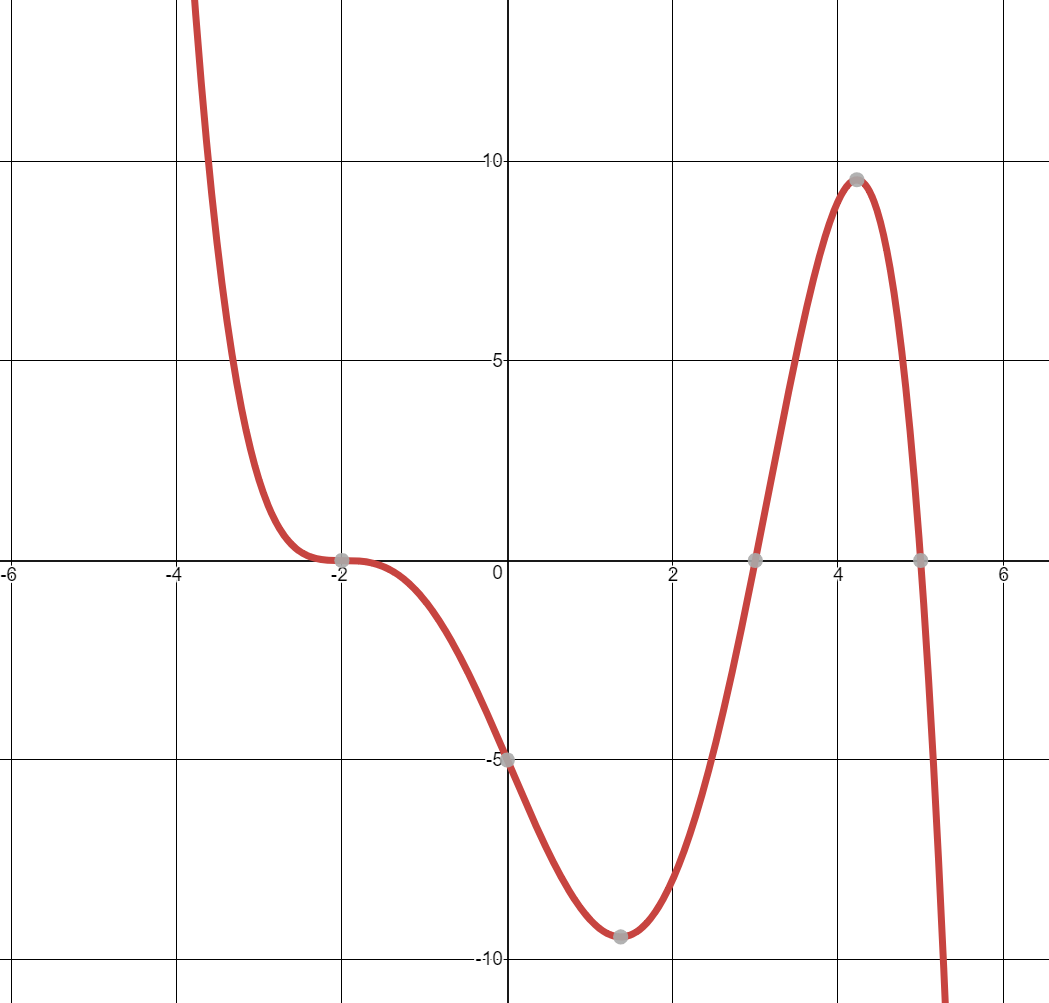
\includegraphics[scale=.35]{p3.png} \end{center}

\begin{center} 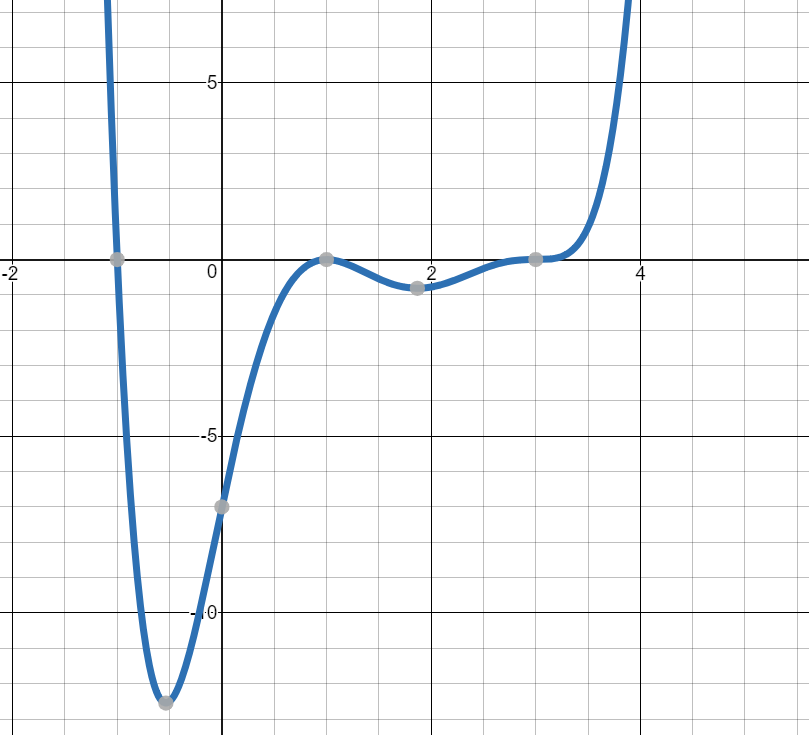
\includegraphics[scale=.45]{p4.png} \end{center}
\eq

\section{Rational Polynomials and Their Graphs}
Big Ideas:
\begin{itemize}
\item Understand the additional features that rational polynomials have
\item Efficiently graph rational polynomials using:
\subitem Intercepts (including the behavior at $x$-intercepts)
\subitem End behaviors (including horizontal and slant asymptotes)
\subitem Vertical asymptotes
\end{itemize}
\begin{info} Rational polynomial functions are of the form $y =\frac{f(x)}{g(x)}$, where $f$ and $g$ are polynomials in $x$. Rational comes from the same root word as ratio, so rational polynomials are \underline{ratios} of polynomials. Rational polynomials have many of the same behaviors as polynomials, such as $x-$ and $y-$ intercepts, right and left end behaviors, etc. One of the features that rational polynomials can have that do not occur in polynomials are asymptotes (vertical, horizontal, or slant).\end{info}
\bq Give all intercepts for the following rational polynomials:
\be
\item $y=\frac{x^2-1}{x^2+1}$
\item $y=\frac{1-x^2}{3x+1}$
\item $y=\frac{x^3-125}{2x-1}$
\item $y=\frac{5x}{(x-1)^2(3x+1)}$
\item $y=\frac{x^2+4x+4}{(x-2)^2}$
\item $y=\frac{x^2+4x+4}{x-2}$
\item $y=\frac{x-2}{x^2+4x+4}$
\ee
\eq

\bq Draw the graphs for the following basic rational polynomials on the same set of axes below:
$$ y=1/x,\quad y=1/x^2, \quad y=1/x^3, \quad y=1/x^4$$

\begin{center} \includegraphics[scale=.5]{unitaxes.png} \end{center}

\be
\item What patterns do you see for the end behavior? Do even degrees still have the same behavior on both sides? Do odd degrees have opposite behaviors?
\item What patterns do you see for the behavior around $x=0$? Do even degrees still have the same behavior on both sides? Do odd degrees have opposite behaviors?
\ee
\eq

\begin{info}
A rational polynomial of the form $y =\frac{f(x)}{g(x)}$ will have a vertical asymptote at $x=a$ if $g(a)=0$ and $f(a) \neq 0$. Vertical asymptotes have multiplicity the same way that $x$-intercepts do and you can determine the directions (same or opposite) in which the asymptote will be approached in the same way. In other words, a vertical asymptote $x=a$ coming from a term of multiplicity $k$ (the factor will look like $(x-a)^k$) will behave like $1/x^k$ does around $x=0$. The graph of a rational polynomial should \textbf{NOT} intersect a vertical asymptote since the denominator of the rational polynomial is zero at the $x$-value given by the vertical asymptote.

\begin{center} \includegraphics[scale=.75]{vaeven.png} \includegraphics[scale=.75]{vaodd.png} \end{center}
\end{info}
\bq Give all vertical asymptotes (and their multiplicity) for the following rational polynomials:
\be
\item $y=\frac{x^2-1}{x^2+1}$
\item $y=\frac{1-x^2}{3x+1}$
\item $y=\frac{x^3-125}{2x-1}$
\item $y=\frac{5x}{(x-1)^2(3x+1)}$
\item $y=\frac{x^2+4x+4}{(x-2)^2}$
\item $y=\frac{x^2+4x+4}{x-2}$
\item $y=\frac{x-2}{x^2+4x+4}$
\ee
\eq

\begin{info}
Horizontal and slant asymptotes describe some of the \underline{possible} end behaviors of rational polynomials. Because we are trying to describe end behavior, we need to look at the highest degree terms, specifically the \textbf{ratio of the highest degree terms} in the numerator and denominator. The ratio of the highest degree terms is different than the ratio of the degree of the numerator to the degree of the denominator.

Similar to a polynomial, a rational polynomial will have the same end behavior as the ratio of its highest degree terms. Horizontal asymptotes correspond to horizontal (or constant) behavior on the ends and slant asymptotes correspond to slanted (non-horizontal) linear behavior on the ends. If you find that the graph has a slant asymptote, then you need to perform polynomial division to find the slant asymptote.

\begin{center}
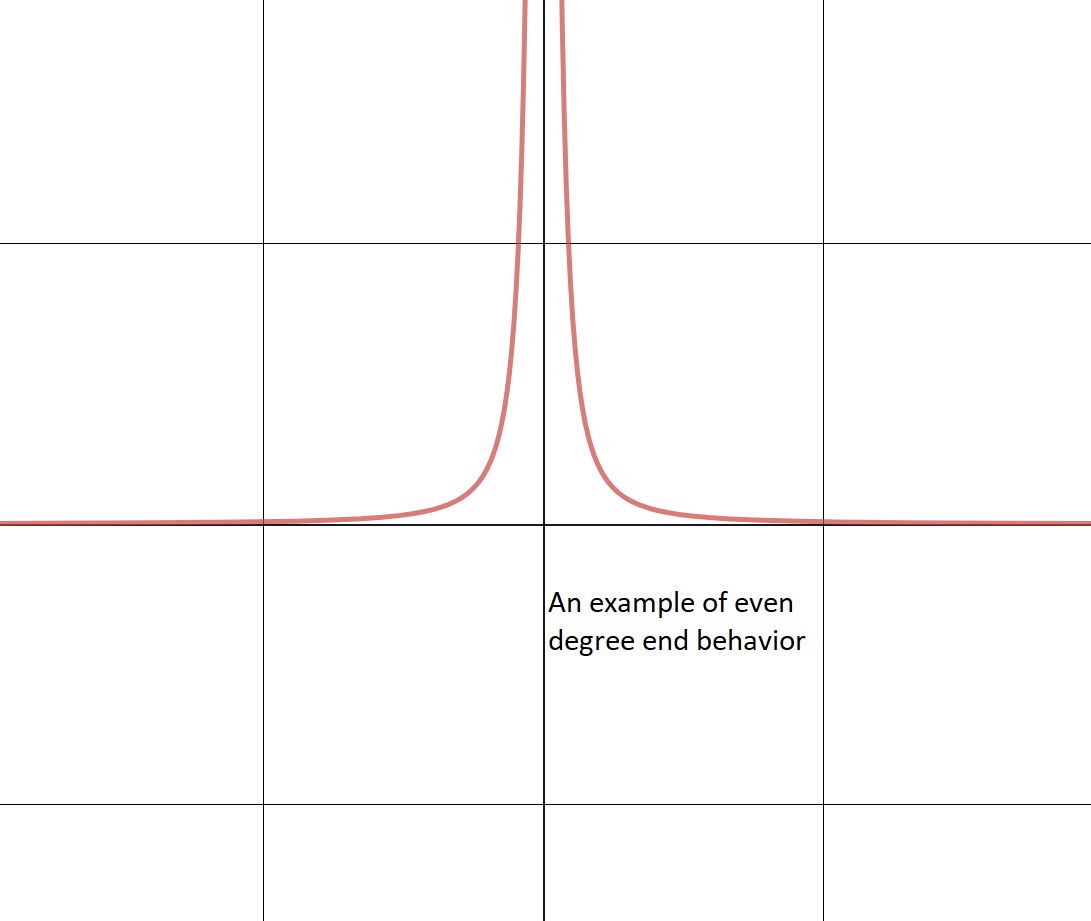
\includegraphics[scale=.35]{even_horiz_asymp_example.png}

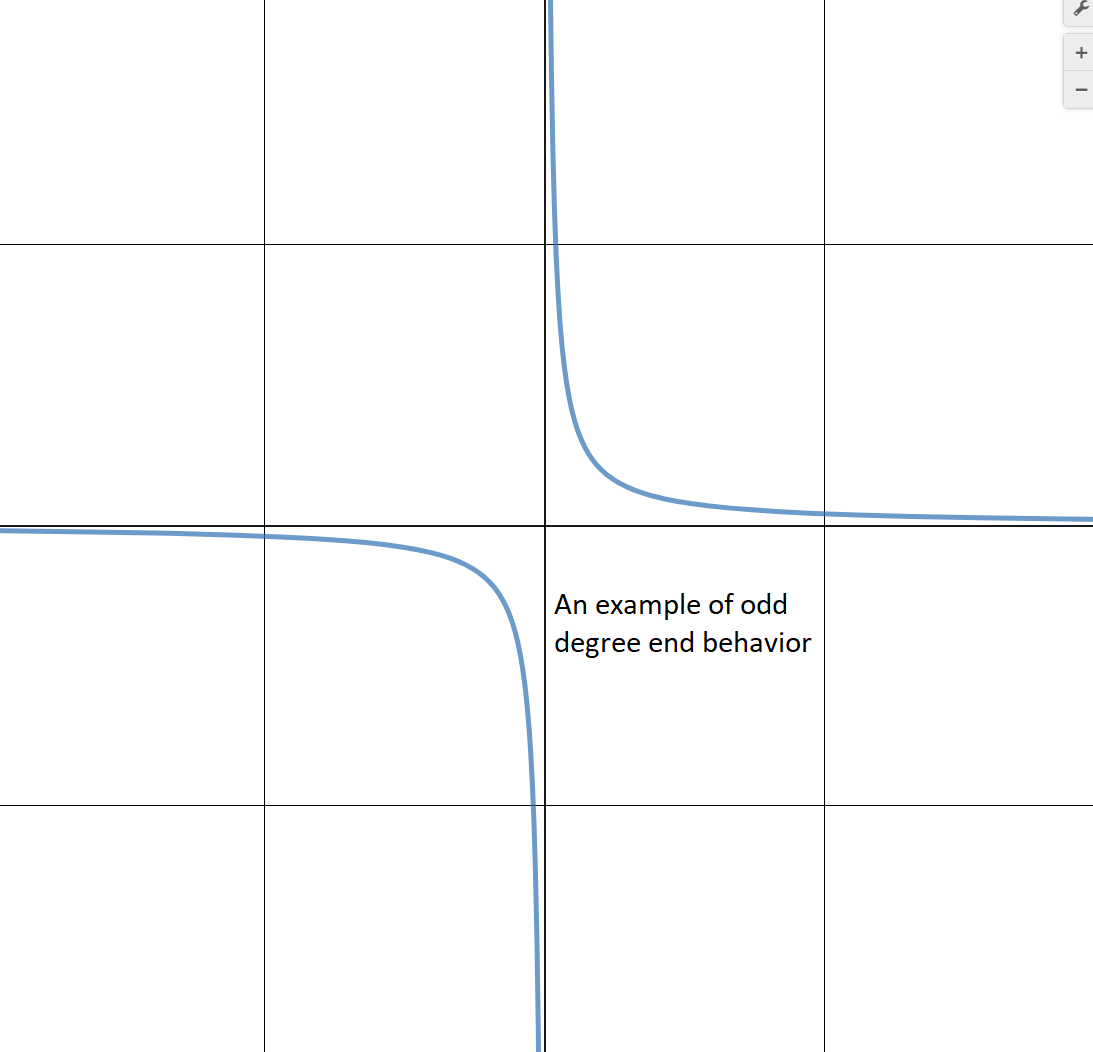
\includegraphics[scale=.35]{odd_horiz_asymp_example.png}

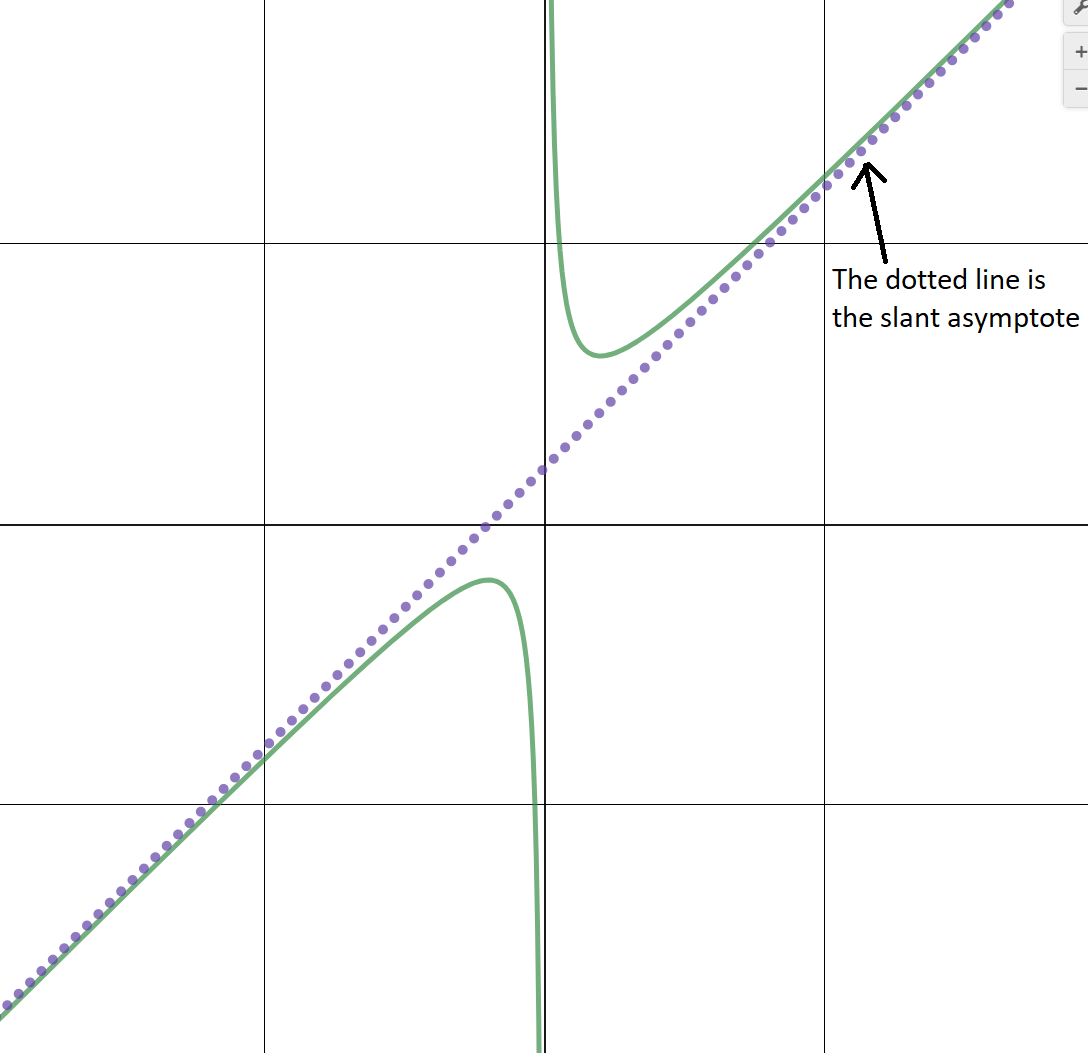
\includegraphics[scale=.35]{slant_asymp_example.png}
\end{center}
\end{info}

\bq Answer all of the questions based on the following graph of a rational polynomial.
\begin{center} \includegraphics[scale=.45]{r1.png} \end{center}
\be
\item List out all vertical asymptotes of the rational polynomial and their multiplicities.
\item Give all intercepts (both $x$ and $y$) for the rational polynomial.
\item What line does this graph have as an end behavior? In other words, what line does this graph approach as you go off the ends of the graph. It may be helpful to cover up the middle part of the graph (from -4 to 4 in $x$) to look at the end behavior.
\ee
\eq
As the previous problem shows, horizontal asymptotes can cross the graph of a rational polynomial because horizontal (and slant) asymptotes only describe the behavior of the graph on the right and left edges and do not tell us what is happening in the middle of the graph.

\bq Answer all of the questions based on the following graph of a rational polynomial.
\begin{center} \includegraphics[scale=.45]{r2.png} \end{center}
\be
\item List out all vertical asymptotes of the rational polynomial and their multiplicities.
\item Give all intercepts (both $x$ and $y$) for the rational polynomial.
\item What line does this graph have as an end behavior? In other words, what line does this graph approach as you go off the ends of the graph. It may be helpful to cover up the middle part of the graph(from -4 to 4 in $x$) to look at the end behavior.
\ee
\eq
The previous problem shows how the end behavior of a rational polynomial can be a slanted line. As you will see over the next several problems, rational polynomials can have only one of the following possibilities: a horizontal asymptote, a slant asymptote, or neither.

\bq For each of the following graphs,
\be
\item State all vertical asymptotes and their multiplicities
\item State all $x$- and $y$- intercepts (including multiplicities for $x$-intercepts).
\item State if the graph has a horizontal asymptote, slant asymptote, or neither. Give the equation of the horizontal or slant asymptote, if they exist.
\ee
\begin{center} \includegraphics[scale=.45]{r3.png}

\includegraphics[scale=.40]{r4.png}

\includegraphics[scale=.40]{r5.png} \end{center}

\eq

\bq \be
\item What is the ratio of the highest degree terms for the following rational polynomials?
\item Simplify the ratio of the highest degree terms. What will the end behavior of this simplified expression be?
\item What is the right and left end behavior? In other words, what horizontal or slant asymptotes will the graph have? Remember that if you have a slant asymptote, you will need to perform polynomial long division on the rational polynomial to find the equation of the slant asymptote.
\ee
\be
\item $y=\frac{x^2-1}{x^2+1}$
\item $y=\frac{1-x^2}{3x+1}$
\item $y=\frac{x^3-125}{2x-1}$
\item $y=\frac{5x}{(x-1)^2(3x+1)}$
\item $y=\frac{x^2+4x+4}{(x-2)^2}$
\item $y=\frac{x^2+4x+4}{x-2}$
\item $y=\frac{x-2}{x^2+4x+4}$
\ee
\eq

\bq Using the information you computed in the questions of this section, draw the graphs of the following rational polynomials. Be sure to label \textbf{all} intercepts, asymptotes and other features of your graph.
\be
\item $y=\frac{x^2-1}{x^2+1}$
\item $y=\frac{1-x^2}{3x+1}$
\item $y=\frac{x^3-125}{2x-1}$
\item $y=\frac{5x}{(x-1)^2(3x+1)}$
\item $y=\frac{x^2+4x+4}{(x-2)^2}$
\item $y=\frac{x^2+4x+4}{x-2}$
\item $y=\frac{x-2}{x^2+4x+4}$
\ee
\eq
\newpage

\chapter{The General Second Degree Equation and Conic Sections}

\begin{annotation}
\endnote{I would suggest doing a simple motivating problem here. My suggestion is as follows:
-Ask students to graph $3x+2y-4=0$. \newline
-Walk around to small groups while they do this problem noting how they approach this. Almost all students (perhaps unconsciously) do the following: \newline
-They identify the shape of the graph should be a line.\newline
-They plot the graph using a minimal set of information (namely two points, then connect and extend)\newline
-This is where you can have them go the other way (find an equation for the line in a given picture) or go right into talking about building the correspondences between algebraic forms and minimal geometric information for graphing.\newline
-This last chapter is about understanding some semi-familiar shapes and the algebraic/geometric forms of those shapes.}
\end{annotation}

\begin{info} Previously, we had the general form of a line as given by the general 1st degree equation: $$Ax+By+C=0$$

In this chapter, we will be looking at the \textbf{general second degree equation}: $$Ax^2+Bxy+Cy^2+Dx+Ey+F=0$$

The possible graphs of the general second degree equation are called conic sections.
\begin{center}\includegraphics[scale=.5]{conics.png}

Credit: The Open University \begin{annotation}
\endnote{\verb{https://www.open.edu/openlearn/ocw/pluginfile.php/89406/mod_oucontent/oucontent/741/f381702f/158b2302/m208_1_i057i.jpg}}

\end{annotation}
\end{center}
\end{info}
\section{Circles}
Big Ideas:
\begin{itemize}
\item Identify the equation of a circle
\item Identify the center and radius of a circle given the general form of a circle.
\end{itemize}
\begin{info} A circle is the set of all points in a plane at a fixed distance (called the radius) from a fixed point (called the center).
\end{info}
\bq
\be
\item What is the distance from $(x,y)$ to $(-3,7)$?
\item Let $C_1$ be the circle with center $(-3,7)$ and radius $4$. If $(x,y)$ is on $C_1$, what should the distance from part $a)$ equal?
\item Use your previous answer to give an equation of the circle $C_1$. Your answer should have a square root in it.
\item Simplify your answer to the previous part by getting rid of the square root but do not expand any other terms.
\ee \eq
Note that if your simplified equation had a center of $(h,k)$ and radius of $R$, the equation would be $$(x-h)^+(y-k)^2=R^2$$ This is called the \textbf{Standard Form of a Circle}.

Given a general 2nd degree equation, we would like to tell when we have a circle or not \underline{without} having to graph it. Ideally, we want to identify the shape of the graph from a simple rule based on the equation you are given.

\bq Expand the Standard Form of a Circle into a general second degree equation of the form $Ax^2+Bxy+Cy^2+Dx+Ey+F=0$. Be sure to combine all like terms so you can compare your expanded Standard Form of a Circle to the general second degree equation. Don't worry about how $R$, $h$, and $k$ are related to $A$, $B$, etc. What pattern can you see in how a circle can be written in general 2nd degree form? What terms are missing?
\eq

\bq For each of the following general 2nd degree equations, state whether the graph can be a circle? Hint: Apply the patterns you saw in the previous question to decide whether the graph is a circle or not.
\be
\item $3x^2+4xy+3y^2-2x+4y-10=0$
\item $3x^2+3y^2-2x+4y-10=0$
\item $3x^2-3y^2-2x+4y-10=0$
\item $3x^2-2x+4y-10=0$
\item $4x+y^2+2x^2-2y=0$
\ee
\eq

Remember our earlier discussion about how to complete the square from Chapter 1. Completing the square will be necessary to convert general 2nd degree equations to the standard form of a circle.

\bq What is the center and radius of the circle given by $2x^2+2y^2-4x+10y-10=0$? Give a graph.
\eq
\bq What is the center and radius of the circle given by $2x^2+2y^2-4x+10y+20=0$? Give a graph.
\eq
\bq What is the center and radius of the circle given by $2x^2+2y^2-4x+10y+\frac{29}{2}=0$? Give a graph.
\eq
\section{Parabolas}
Big Ideas:
\begin{itemize}
\item Understand how the definition of a parabola gives the standard form of a parabola
\item Identify and apply the standard from of a parabola to algebraic and word problems.
\item Understand and be able to label the important graphical features of a parabola including the focus, the vertex, and the directrix.
\end{itemize}
Just like our previous shapes (lines, polynomials, rational polynomials, circles), we want to find some algbraic form that helps us figure out the graph or important points in the geometry.
\begin{info}
A \textbf{parabola} is the set of all points in a plane equidistant from a fixed point (called the focus)  and a fixed line (called the directrix)

In other words, points on the parabola should be the same distance away from the directrix as they are from the focus.
\end{info}

\begin{center}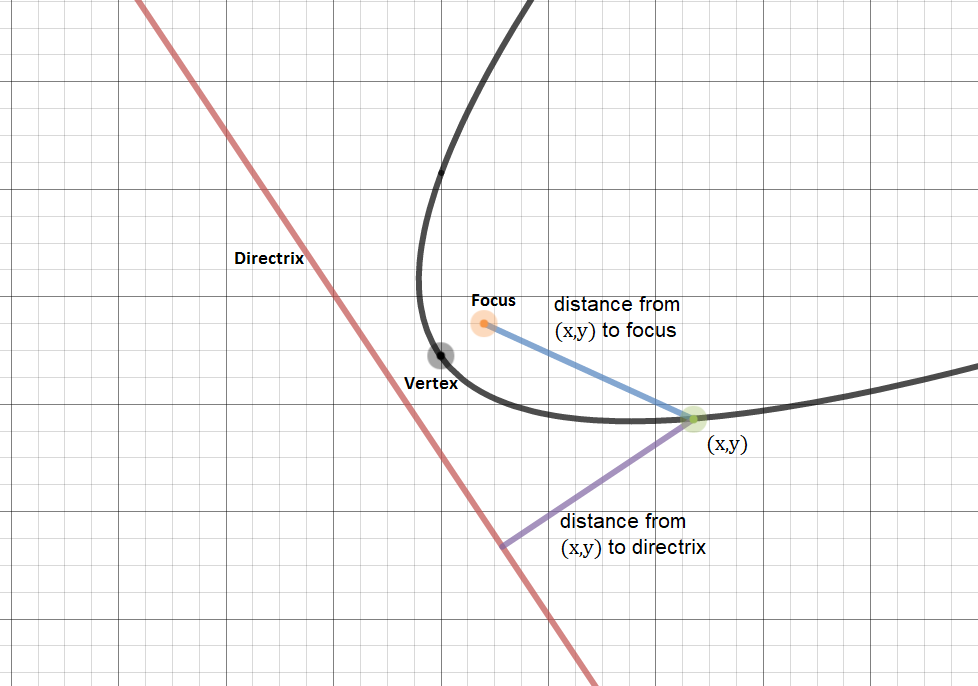
\includegraphics[scale=.45]{generalparabola2.png} \end{center}

In the next question we will use the definition of a parabola to get the standard form of a parabola.

\begin{annotation}
\endnote{Remind students here that without Question \ref{q22}, they can't do any of the problems in this section. I will often do Question \ref{q22} as a class (let them work, pull together for a quick class discussion; or have them work in groups on the algebra at the boards so everyone can see how to write things up).}
\end{annotation}

\bq\label{q22} \be
\item On the same set of axes, graph the point $(c,0)$ and $x=-c$.
\item What is the distance from the point $(x,y)$ to the point $(c,0)$?
\item What is the distance from the point $(x,y)$ to the line $x=-c$?
\item Use your answer to the previous parts to give the equation of a\break parabola with focus $(c,0)$ and directrix given by $x= -c$.
\item Simplify the equation of the parabola as much as possible. This will require some algebra but we should have a nice form to use for parabolas of this type and we will not need to do this algebra again for a parabola. Hint: Solve for $y^2$ at the end.
\item Fill in your graph from part a) with the graph of the parabola with focus $(c,0)$ and directrix $x= -c$.
\ee \eq
Notice that in the previous problem, the focus is on the $x$ axis, the directrix is of the form $x=$ a constant, the linear term in the standard form is $x$, and the parabola opens in the $x$ direction (either right or left depending on the sign of $c$).

\question\label{q23} How would your equation change if the focus of a parabola is at the point $(0,c)$ and the directrix is given by $y=-c$? Hint: We have just switched the roles of the $x$ and $y$ coordinates...

\begin{info} A conic section in \textbf{standard position} means that the focus (or foci) is on either the x- or y-axis and the center is at the origin. This definition applies to parabolas, ellipses, and hyperbolas.

For a parabola, the \textbf{vertex} and the \textbf{center} are \emph{the same point} and $c$ is the distance from the center to the focus. You should not think of $c$ as being the coordinate of the focus since not every parabola we will deal with is in standard position. When plotting a parabola, you need to label the \underline{focus}, the \underline{directrix}, and the \underline{vertex}.

\begin{center} 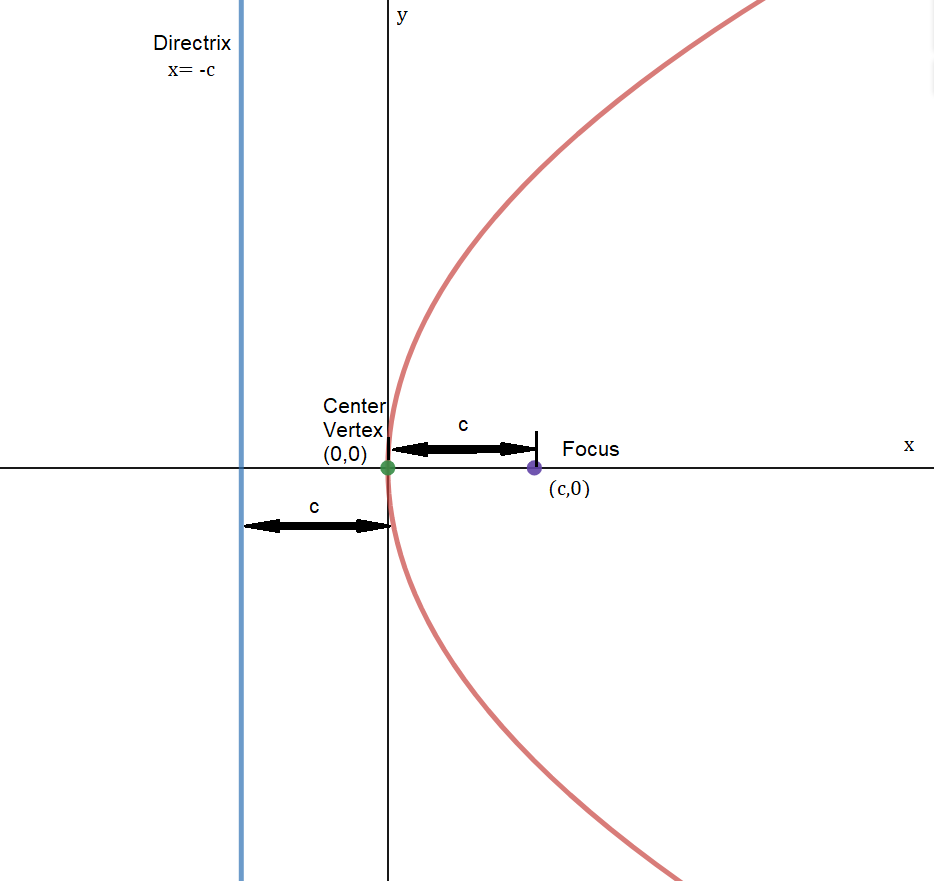
\includegraphics[scale=.4]{parabolasp3.png} \end{center}

Note that the forms you found in Questions \ref{q22} and \ref{q23} will work for negative values of $c$ as well.
\end{info}

\bq
\be
\item What value of $c$ will make $y=x^2$ fit the forms you just found?
\item Graph $y=x^2$. Be sure to include the focus and directrix on your graph.
\ee
\eq

\question Graph $y^2=-3x$.

\question What is the equation of the parabola in \underline{standard position} with focus $(0,-6)$? What is $c$ for this problem?

\question Give the equations of \textbf{all} parabolas in standard position that contain the point $(2,4)$. Hint: There are two answers to this problem.

\question Give the equations of all parabolas in standard position that contain the points $(3,-4)$ and $(-3,-4)$

\begin{info} Parabolas have many uses including as reflectors, as bridge supports, and in celestial mechanics. For instance, parallel beams of incoming light or sound will be reflected by a parabolic mirror through the focus.

\begin{center} 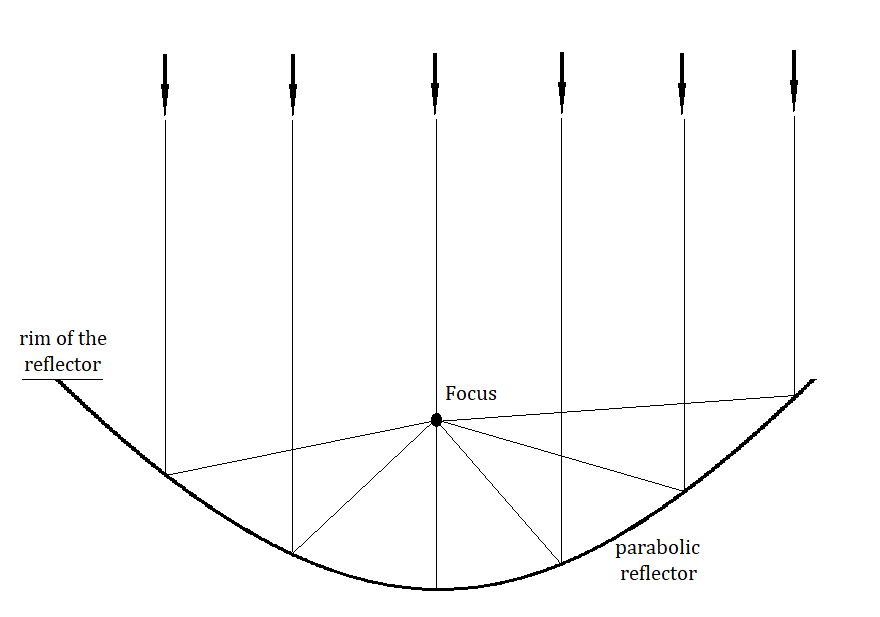
\includegraphics[scale=.4]{parabolic-reflector2.png} \end{center}

When solving application/word problems make sure you draw a good picture and label all of the information you have before you try to put coordinates to the problem or use an equation.
\end{info}

\question While watching the Dallas Cowboys play the New England Patriots, you notice that the Patriots are using a parabolic reflector with a microphone at its focus to spy on Jerry Jones' drink orders. You notice that the microphone is in the same plane as the edge of the reflector and the reflector has a diameter of 3.5 feet. How far is the microphone from the vertex of the reflector? Hint: Draw a picture and carefully label the information given in the problem. Put a convienent coordinate system on your picture and then use the algebraic forms from above.

\question Later in the game you see another parabolic reflector being used to spy on Tony Romo's wife but this time you can tell that the microphone is in the same plane as the edge of the reflector and that the microphone is 8 inches from the vertex of the reflector. How wide is this second listening device?

\section{Ellipses}
Big Ideas:
\begin{itemize}
\item Understand how the definition of a ellipse gives the standard form of a ellipse.
\item Identify and apply the standard from of a ellipse to algebraic and word problems.
\item Understand and be able to label the important graphical features of a ellipse including the center, the foci, the vertices, and the covertices.
\end{itemize}
\begin{info} An \textbf{ellipse} is the set of all points, $(x,y)$, such that the sum of the distances from the point $(x,y)$ to a pair of distinct points (called foci) is a fixed constant. We will call this constant $2a$.
\end{info}
\begin{center} 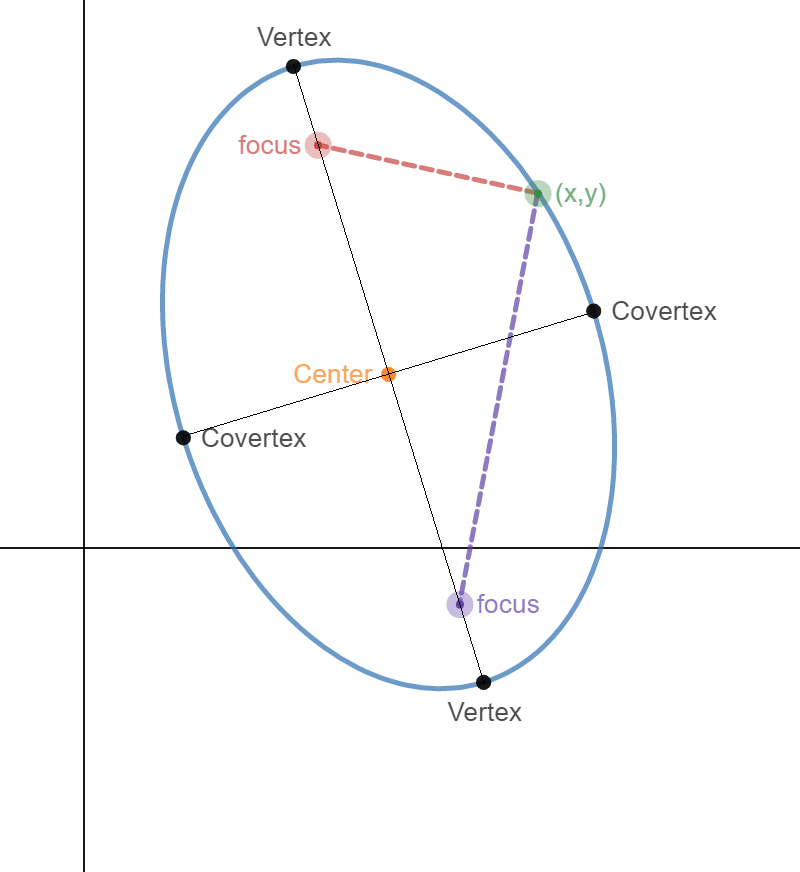
\includegraphics[scale=.45]{generalellipse3.png} \end{center}
This graph shows an ellipse with the dotted lines showing the distances from $(x,y)$ to each of the foci. This ellipse is not in standard position but gives you an example of a general ellipse. 

The \lq\lq nice\rq\rq conic sections we will deal with first are in standard position. Standard position means that the focus (or foci) is on either the $x$- or $y$-axis and the center is at the origin.

\bq\label{q62} Let $C_1$ be the ellipse with foci $F_1$ and $F_2$.
\be
\item If $d_1$ is the distance from a point $(x,y)$ to $F_1$, $d_2$ is the distance from a point $(x,y)$ to $F_2$, and the point $(x,y)$ is on $C_1$, how are $d_1$, $d_2$, and $a$ related?
\item What is the distance from a point $(x,y)$ to the point $(c,0)$?
\item What is the distance from a point $(x,y)$ to the point $(-c,0)$?
\item Use your answer to the previous parts to give the equation of an ellipse with foci $(c,0)$ and $(-c,0)$.
\item Simplify your equation as much as possible. This will require some \textbf{\underline{serious}} algebra but we should have a nice form to use for ellipses of this type and we will not need to do this algebra again for an ellipse. Near the end of this algebra you should substitute $b^2$ where you see the factor $a^2-c^2$. We will talk about what $b$ means in the next couple of problems.
\item What are the $x$- and $y$-intercepts for this ellipse?
\ee \eq

\begin{annotation}
\endnote{This is a problem that will build and test the students' persistence. You will need to decide how to guide them through some of the algebra in this problem, including the suggestion to move one of the square roots from part d) to the other side of the equation to simplify the algebra). Getting student to do the work here is an important checkpoint to make sure they are ready for the final few sections of problems which will require them to work for more than a few minutes on problems that are not easily solved. You may want to have this be a problem that students work in class and present results as you go.}
\end{annotation}

\bq \be
\item How does your equation change if the foci are $(0,c)$ and $(0,-c)$? Note that this is the same problem as before, just with the foci on the $y$-axis.
\item What are the $x$- and $y$-intercepts for this ellipse?
\ee \eq

\begin{info}
The points on the ellipse farthest from the center on the largest axis (called the major axis) are the \textbf{vertices} and the points on the shorter axis (called the minor axis) are the \textbf{covertices}. The vertices are a distance $a$ from the center and the covertices are a distance $b$ away from the center where $a^2=b^2+c^2$. Remember that $c$ still measures the distance from the center to each focus.

Whenever you draw an ellipse, you need to label the \underline{center}, \underline{foci}, \underline{vertices}, and \underline{covertices}.

The \textbf{eccentricity} of an ellipse is $\frac{c}{a}$. \end{info}
\bq For each of the points, A through H, on the graph below, you need to specify which of the following characteristics applies: Center, Vertex, Focus, Covertex, None of the Above.

What are the values for $a$, $b$, and $c$ for the ellipse in the graph?
\eq
\begin{center} 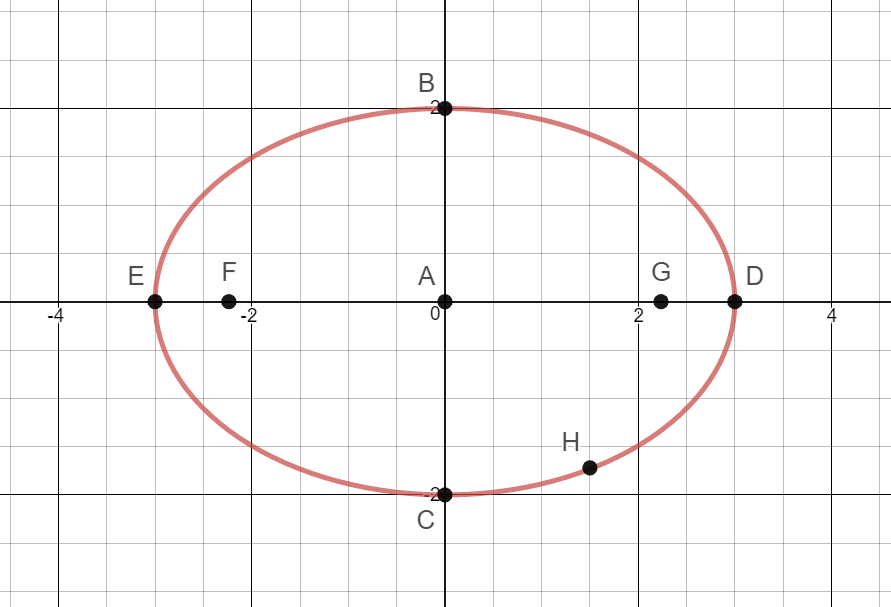
\includegraphics[scale=.5]{ellipse4.png} \end{center}
\bq \be
\item Which of $a$, $b$, or $c$ is associated with vertices?
\item Which of $a$, $b$, or $c$ is associated with covertices?
\item Which of $a$, $b$, or $c$ is associated with foci?
\item If $a^2=b^2+c^2$, which of $a$, $b$, or $c$ has to be the largest? Explain your reasoning.
\item Given that $a^2=b^2+c^2$ for an ellipse, which of the vertices, covertices, or foci are farthest from the center? \ee \eq

\bq Sketch and label the graph of $25x^2+16y^2=400$. You should convert this equation to be in the form given in Question \ref{q62}, then use the information you can get from $a$, $b$, and $c$ to draw your graph and label the center, foci, vertices, and covertices.
\eq
\bq Find an equation of an ellipse with vertices $(\pm 6,0)$ and eccentricity $3/5$. \eq

\bq Sketch and label the graph of $9x^2+y^2=36$. \eq

\bq Find an equation of an ellipse in standard position with vertex $(5,0)$ and contains the point $(\sqrt{15},2)$ \eq

\begin{center} \includegraphics[scale=.4]{ellipse2.png} \end{center}
\bq\label{eq1}
\be
\item What point on the ellipse above is closest to $F_1$?
\item What point on the ellipse above is farthest from $F_1$?
\ee
\eq
\begin{info} Ellipses are used as reflectors and can be found in applications like planetary motion. For instance, the orbit of the Moon around Earth is an ellipse with the Earth at one of the foci and \underline{not} at the center. Ellipses are useful as reflectors because any source of light or sound at one foci will be reflected directly at the other focus. \end{info}

\bq A room is elliptic with vertical walls 6 feet high and an ellipsoid ceiling. If it is 40 feet long and 20 feet wide, where should two people stand (other than next to each other) so that they can whisper to each other without being heard by others in the room? Hint: Sound from one focus will be reflected by the walls to the other focus.
\eq

\bq If the orbit of the Moon around the Earth varies from \break221,463 miles to 252,710 miles, find the eccentricity of the Moon's orbit and the lengths of the major and minor axes. Note that the distances given are not $a$ and $b$ (Hint: Use Question \ref{eq1}).
\eq

\bq The ellipse in Washington DC is 3525 feet by 1265 feet. Give an equation for the edge of the ellipse if the axes are placed in the center with the \underline{$y$-axis as the major axis}. \eq

\section{Hyperbolas}
Big Ideas:
\begin{itemize}
\item Understand how the definition of a hyperbola gives the standard form of a hyperbola.
\item Identify and apply the standard from of a hyperbola to algebraic and word problems.
\item Understand and be able to label the important graphical features of a hyperbola including the center, the foci, the vertices, and the asymptotes.
\end{itemize}

\begin{center} \includegraphics[scale=.5]{generalhyperbola2.png} \end{center}

\begin{info} A \textbf{hyperbola} is the set of all points $(x,y)$ in a plane such that the positive difference  between the distances from $(x,y)$ to a pair of distinct fixed points (called foci) is a fixed constant. Again, we will call this fixed constant $2a$.
Remember:  The \lq\lq nice\rq\rq conic sections we will deal with first are in standard position.
Standard position means that the focus (or foci) is on either the $x$- or $y$-axis and the center is at the origin. Is the hyperbola pictured above in standard position? Why or why not?
\end{info}

\bq \label{q61} Let $C_1$ be the hyperbola with foci $F_1$ and $F_2$.
\be
\item If $d_1$ is the distance from a point $(x,y)$ to $F_1$, $d_2$ is the distance from a point $(x,y)$ to $F_2$, and the point $(x,y)$ is on $C_1$, how are $a$, $d_1$, and $d_2$ related?
\item What is the distance from a point $(x,y)$ to the point $(c,0)$?
\item What is the distance from a point $(x,y)$ to the point $(-c,0)$?
\item Use your answers from the previous parts to give the equation of a hyperbola with foci $(c,0)$ and $(-c,0)$. Leave your answer in terms of the difference of square root terms. 
\item Simplify your equation as much as possible. This will require some serious algebra but we should have a nice form to use for hyperbolas of this type and we will not need to do this algebra again. Near the end of this algebra you should substitute in $b^2$ in where you see the factor $c^2-a^2$ (This is different than what we found for an ellipse). We will talk about what $b$ means in the next couple of problems.
\item What are the $x$- and $y$-intercepts for this hyperbola?
\ee \eq

\begin{annotation}
\endnote{I will often do Question \ref{q61} (just like Question \ref{q22}) as a class (let them work, pull together for a quick class discussion; or have them work in groups on the algebra at the boards so everyone can see how to write things up).}
\end{annotation}

\bq \be
\item How does your equation from Question \ref{q61} part e) change if the foci are $(0,c)$ and $(0,-c)$?
\item What are the $x$- and $y$-intercepts for the hyperbola with foci $(0,c)$ and $(0,-c)$?
\ee \eq

\begin{info}
The points on the hyperbola closest to the center (on the major axis) are the \textbf{vertices}. The vertices are a distance $a$ from the center and the \textbf{asymptotes} are of the form $y=\pm(\frac{a}{b}) x$ (if foci are on the $y$-axis) or $y=\pm(\frac{b}{a}) x$ (if foci are on the $x$-axis) where $a^2+b^2=c^2$.

Whenever you draw a hyperbola, you need to label the \underline{center}, \underline{foci}, \underline{vertices}, and \underline{asymptotes}.

The \textbf{eccentricity} of a hyperbola is $\frac{c}{a}$. \end{info}

\bq Give the values of $a$, $b$, and $c$ for each of the following hyperbolas.
\be
\item $\frac{x^2}{16}-\frac{y^2}{25}=1$
\item $\frac{x^2}{25}-\frac{y^2}{16}=1$
\item $\frac{y^2}{16}-\frac{x^2}{25}=1$
\ee
\eq

\bq Sketch and label the graph of $25x^2-16y^2=400$. \eq

\bq Give the equation of a hyperbola with vertices $(0,\pm3)$ and $e=5/3$ \eq

\bq Sketch and label the graph of $9x^2-y^2=-36$. \eq

\bq  A proton is launched along the line $y = \frac{1}{2} x$ toward the nucleus of an atom at the origin. If the proton is deflected upwards toward the line $y = -\frac{1}{2} x$ along a hyperbolic path, give the equation for the path of the proton. Hint: Draw all the ways the proton could approach the origin along the line $y=\frac{1}{2} x$ and be deflected toward the line $y =-\frac{1}{2} x$. There should be 4 possibilities. Which of the possibilities is described above? \eq

\bq Repeat the previous problem if the proton is deflected downward toward the line $y = -\frac{1}{2} x$ along a hyperbolic path. \eq

\bq A person standing at a point $Q=(x,y)$ hears the crack of a rifle at point $P_1= (1000,0)$ and the sound of the bullet hitting the target at $P_2=(-1000,0)$ at the same time. The bullet travels at 2000 ft/s and sound travels at 1100 ft/s. We want to find an equation relating $x$ and $y$.
\be
\item Draw a graph with the points $Q$, $P_1$ and $P_2$ labeled.
\item Find $t_1$, the time it takes the bullet to go from the rifle to the target. (Remember that $time = \frac{distance}{speed}$)
\item Find $t_2$, the time it takes the sound of the gun to reach the person at $Q$.
\item Find $t_3$, the time it takes the sound of the target being hit to reach the person at $Q$.
\item How are $t_1$, $t_2$, and $t_3$ related?
\item Use your answers to the previous questions to find an equation relating $x$ and $y$.
\ee
\eq

\section{Translated Conic Sections}
Big Ideas:
\begin{itemize}
\item Review translation of coordinates
\item Understand (geometrically and algebraically) when conic sections can be translated to standard position
\end{itemize}

\bq \label{q32} \underline{Summary Question:}

\be
\item Write out the forms of a parabola in standard position (there should be two). For each form, give the focus, the directrix, and the vertex.
\item Write a sentence that describes what $c$ measures for a parabola.
\item How far is the center from the vertex in a parabola?
\item Write out the forms of an ellipse in standard position (there should be two). For each form, give the foci, the vertices, and the covertices.
\item Write a sentence that describes what $a$, $b$, and $c$ measures for an ellipse.
\item How are $a$, $b$, and $c$ related for an ellipse? Which is the largest?
\item Write out the forms of a hyperbola in standard position (there should be two). For each form, give the foci, the vertices, and the asymptotes.
\item Write a sentence that describes what $a$, $b$, and $c$ measures for a hyperbola.
\item How are $a$, $b$, and $c$ related for a hyperbola? Which is the largest?
\ee \eq

\bq For each of the shapes below:
\be
\item Give the coordinates for the center of the conic section.
\item In a new \underline{color}, draw a new set of axes through the \textbf{center} of the conic section and label them $\hat{x}$ and $\hat{y}$.
\item Write the equation of the conic section in terms of the $\hat{x}-$ and $\hat{y}-$ coordinates. Hint: In terms of $\hat{x}$ and $\hat{y}$, the conic section is in standard position and you can use the forms from Question \ref{q32}.
\item Recall from Questions \ref{q30} and \ref{q31} that if the origin of the $\hat{x}\hat{y}-$axes has coordinates  $(h,k)$ in terms of the $xy-$axes, then $\hat{x} =x-h$ and $\hat{y}=y-k$. Use these ideas to write the equation of the conic section in terms of the $x$- and $y$-axes. Hint: Look at part a) to get the values for $h$ and $k$.
\ee
\begin{center}\includegraphics[scale=.8]{ellipse1.png}

\includegraphics[scale=.75]{hyperbola1.png}

\includegraphics[scale=.75]{parabola1.png} \end{center}
\eq
In the next problem, we will write out \underline{all} of the translated conic section forms.
\bq \be
\item Write out the form of a parabola that has center $(h,k)$ and opens left or right. Give the focus, the directrix, and the vertex.
\item Write out the form of a parabola that has center $(h,k)$ and opens up or down. Give the focus, the directrix, and the vertex.
\item Write out the form of an ellipse that has center $(h,k)$ and its major axis moves left/right. Give the foci, the vertices, and the covertices.
\item Write out the form of an ellipse that has center $(h,k)$ and its major axis moves up/down. Give the foci, the vertices, and the covertices.
\item Write out the form of a hyperbola that has center $(h,k)$ and opens left/right. Give the foci, vertices, and asymptotes.
\item Write out the form of a hyperbola that has center $(h,k)$ and opens up/down. Give the foci, vertices, and asymptotes.
\ee
\eq

\bq For each of the forms in the previous question, expand each of the forms  and compare the results to the general second degree equation ($Ax^2+Bxy+Cy^2+Dx+Ey+F=0$). What kinds of terms do you notice? Which terms are missing? Which terms can have the same or opposite signs? Just like we talked about with circles, the goal of this exercise is to be given a general second degree equation of the form, $Ax^2+Bxy+Cy^2+Dx+Ey+F=0$, and identify if the graph will be one of the translated conic sections.

For example, the form $(y-k)^2=4c(x-h)$ will have a $y^2$-term but not $x^2$ and $xy$-terms. In other words, $A=B=0$ and $C\neq 0$. \eq

\bq For each of the following general second degree equations, identify what type of conic section is represented and complete the square or factor as necessary to obtain the translated form of the conic section. If it is not possible to identify the type of conic section, state why you can't identify the shape of the graph.
\be
\item $x^2-8x-8y+8=0$
\item $x^2-xy+y^2-2=0$
\item $4x^2+y^2+24x-2y+21=0$
\item $9x^2-4y^2+90x+32y+125=0$
\item $x^2+4xy-2y^2-6=0$
\ee
\eq

\section{Rotated Conic Sections}
Big Ideas:
\begin{itemize}
\item Identify both algebraically and geometrically, when rotation of coordinates are necessary
\item Algebraically perform rotation of coordinates to get a conic section in standard position.
\end{itemize}
\bq
Answer the following questions for the ellipse graphed below
\begin{center} \includegraphics[scale=.5]{ellipserot.png} \end{center}
\be
\item Draw the major and minor axes on the graph of the ellipse.
\item What is the center of the ellipse?
\item Will translating coordinates (without any other changes) put the ellipse into standard position? Why or why not?
\ee
\eq

\begin{info} In our previous problems, we saw how translating our coordinate system to the center of our figure ($\hat{x}=x-h$ and $\hat{y}=y-k$) simplified our problem to standard position.

We still have to find equations and graph conics that are not oriented up/down or left/right. For this we will need to look at rotated coordinate systems. Specifically, if we would like to rotate our coordinate system counterclockwise by $\theta$ around the origin, we use the substitution 
$$x=\hat{x} \enskip \cos(\theta) - \hat{y} \enskip \sin(\theta) $$ $$y=\hat{x} \enskip \sin(\theta) + \hat{y} \enskip \cos(\theta)$$

\begin{center} \includegraphics{rotation.png} \end{center}
\end{info}
\bq \be
\item Draw a set of $xy$-axes and in another color draw $\hat{x}\hat{y}$-axes which are given by a rotation of $\frac{\pi}{2}$ (counterclockwise).
\item Plug $\theta = \frac{\pi}{2}$ into the coordinate rotation equations given above and simplify.
\item Does your answer from part $b)$ make sense with the geometric picture you drew in part $a)$?
\ee \eq

\bq
\be
\item How far is $y=x+1$ from the origin? Be careful in your answer.
\item Simplify the coordinate rotation equations for $\theta =\frac{\pi}{4}$.
\item Using your simplified coordinate rotation equations from part $a)$, find a new representation of the line $y=x+1$ after rotating by an angle of $\frac{\pi}{4}$. In other words, find a new equation for $y=x+1$ be in terms of $\hat{x}$ and $\hat{y}$.
\item Draw $y=x+1$ on the $xy$-axes.
\item Draw your answer to part $c)$ on a separate plot using $\hat{x}\hat{y}$-axes.
\item Now draw a graph that contains both the $xy$-axes and $\hat{x}\hat{y}$-axes (how are they related?). What does the graph of $y=x+1$ look like on this new plot?
\ee
\eq

\question Find a new representation of $x^2-xy+y^2-2=0$ after rotating by $45^{\circ}$. Is your new rotated conic section in standard position (relative to the $\widehat{x}$ and $\widehat{y}$ coordinates)? If so, graph the conic with both the original and rotated set of axes.

\question Find a new representation for $31x^2+21y^2+10\sqrt{3}xy=144$ after rotating by $\frac{\pi}{3}$. Is your conic section in standard position? If so, graph the conic with both the original and rotated set of axes.

\begin{info} Given a general second degree equation of the form $Ax^2+Bxy+Cy^2+Dx+Ey+F=0$, rotation by an angle $\theta$ that satisfies
$\tan(\theta) = \frac{(C-A)\pm \sqrt{(C-A)^2+B^2}}{B}$ will give a representation without a $xy$-term.
\end{info}

\question What angle of rotation is needed to eliminate the $xy$-term of $x^2-xy+y^2-2=0$?

\question What angle of rotation is needed to eliminate the $xy$-term of $31x^2+10\sqrt{3}xy+21y^2-144=0$?

\question What angle of rotation is needed to eliminate the $xy$-term of $x^2+4xy-2y^2-6=0$?

\question Give the equation of the conic section given by $31x^2+ \break10\sqrt{3}xy +21y^2 =144$ after rotating to eliminate the $xy$-term. Graph the conic with both the original and rotated set of axes.

\question Give the equation of the conic section given by $x^2+4xy-2y^2-6=0$ after rotating to eliminate the $xy$-term. Graph the conic with both the original and rotated set of axes.

\begin{info}
The shape of the conic section with equation $Ax^2+Bxy+Cy^2+Dx+Ey+F=0$ is given by the following table:

\begin{tabular}{| l | l |}
\hline
Conic Section & $B^2-4AC$ \\
\hline
\hline
Hyperbola & Positive \\
Parabola & 0 \\
Ellipse & Negative \\
\hline
\end{tabular}\end{info}


\bq What kind of conic section is:
\be
\item $x^2-xy+y^2-2=0$
\item $31x^2+10\sqrt{3}  xy+21y^2-144=0$
\item $x^2+4xy-2y^2-6=0$?
\item $3x^2-8xy+y^2-9=0$
\item $4x^2+3xy-y^2-9=0$
\item $-2x^2+12xy-18y^2-9=0$
\item $9x^2+8xy-6y^2=70$
\ee
\eq

\section{Other Parametric Forms}
Big Idea:
\begin{itemize}
\item Develop parameterizations of other shapes, including polynomials and conic sections.
\end{itemize}
\begin{info} Recall the equation $(x,y)=(x_1+t(x_2-x_1),y_1+t(y_2-y_1))$ is the \textbf{Parametric Form of a Line} through $(x_1,y_1)$ and $(x_2,y_2)$. We would like to try to describe other shapes using parametric equations. Parametric equations can be given as $x(t)$ and $y(t)$ or as a vector valued function $\vec{\textbf{v}}(t)= \langle x(t),y(t)\rangle$.
\end{info}
\bq Graph each of the following parametric equations. It will probably be helpful to calculate the $(x,y)$ points that correspond to several $t$ values like you did in Question \ref{qp}.
\be
\item $(x,y)=(3t-1,4t+2)$
\item $(x,y)=(t-1,t+1)$
\item $(x,y)=(t^2-1,t^2+1)$
\item $(x,y)=( t^2-2t,t)$
\item $(x,y)=(cos(t),tan(t))$
\ee
\eq
Most parameterizations come from adapting a known shape. The next several problems move from a circle to a translated ellipse.

\question Give parametric equations for the circle centered at the origin of radius 1. Be sure to give the bounds of your parameter $t$. Plot your parametric equations to confirm your answer. Hint: Use your trigonometry knowledge to describe $x$ and $y$ values in terms of some other quantity...

\question Give parametric equations for the circle centered at $(h,k)$ of radius 1. Be sure to give the bounds of your parameter $t$. Plot your parametric equations to confirm your answer.

\question Give parametric equations for $\frac{x^2}{4}+\frac{y^2}{9}=1$. Be sure to give the bounds of your parameter $t$. Plot your parametric equations to confirm your answer.

\question Give parametric equations for $\frac{(x-h)^2}{a^2}+\frac{(y-k)^2}{b^2}=1$. Be sure to give the bounds of your parameter $t$. Plot your parametric equations to confirm your answer.

You could also use one of the variables ($x$ or $y$) as your parameter. After setting $x$ or $y$ equal to $t$, you can then solve for the other variable in terms of $t$.

\question Give parametric equations for $y=x^3-x^2$. Be sure to give the bounds of your parameter $t$. Plot your parametric equations to confirm your answer.

\question Give parametric equations for $y=x^2-x^4$. Be sure to give the bounds of your parameter $t$. Plot your parametric equations to confirm your answer.

\question Give parametric equations for $y^2-8x-8y+8=0$. Be sure to give the bounds of your parameter $t$. Plot your parametric equations to confirm your answer.

\question Give parametric equations for the positive branch of $9x^2-4y^2+90x+32y+125=0$. Be sure to give the bounds of your parameter $t$. Plot your parametric equations to confirm your answer.

\backmatter

\begin{annotation}
\chapter{Notes to the Instructor}
\renewcommand\notesname{}
\vspace{-2cm}
\begingroup
%\setlength{\parindent}{0pt}% Don't know what this does.  DMC
\setlength{\parskip}{2ex}
\renewcommand{\enotesize}{\normalsize}
\theendnotes
\endgroup
\end{annotation}

\end{document}
